\documentclass[aspectratio=169,11pt]{beamer}
% ==========================================================================
%  KSA lecture-slide theme  =  stock beamer "Boadilla"  +  KSA colour theme
%  brand colours sampled from the official KSA symbol mark:
%    Deep Prussian Blue  #2E3192   (지성 - intellect)
%    Golden Gray         #D6CBB1   (감성 - sensibility)
%  Engine: XeLaTeX.  Usage:
%    \documentclass[aspectratio=169,11pt]{beamer}
%    % ==========================================================================
%  KSA lecture-slide theme  =  stock beamer "Boadilla"  +  KSA colour theme
%  brand colours sampled from the official KSA symbol mark:
%    Deep Prussian Blue  #2E3192   (지성 - intellect)
%    Golden Gray         #D6CBB1   (감성 - sensibility)
%  Engine: XeLaTeX.  Usage:
%    \documentclass[aspectratio=169,11pt]{beamer}
%    % ==========================================================================
%  KSA lecture-slide theme  =  stock beamer "Boadilla"  +  KSA colour theme
%  brand colours sampled from the official KSA symbol mark:
%    Deep Prussian Blue  #2E3192   (지성 - intellect)
%    Golden Gray         #D6CBB1   (감성 - sensibility)
%  Engine: XeLaTeX.  Usage:
%    \documentclass[aspectratio=169,11pt]{beamer}
%    \input{../theme/ksa-theme.tex}
% ==========================================================================

\usepackage{fontspec}
\usepackage{amsmath,amssymb}
\usepackage{graphicx}
\graphicspath{{figs/}{../figs/}}
\usepackage{booktabs}
\usepackage{listings}

% ---- fonts (no ctex/xeCJK on this box -> fontspec drives CJK directly) -----
\defaultfontfeatures{Ligatures=TeX}
\setmainfont{Noto Sans CJK KR}
\setsansfont{Noto Sans CJK KR}
\setmonofont{Noto Sans Mono CJK KR}[Scale=0.92]

% ---- base theme: stock Boadilla ------------------------------------------
\usetheme{Boadilla}
\usefonttheme{professionalfonts}
\setbeamertemplate{navigation symbols}{}

% ---- KSA colour theme (recolour the stock theme) --------------------------
\definecolor{ksablue}{HTML}{2E3192}
\definecolor{ksabluedk}{HTML}{20226A}
\definecolor{ksagold}{HTML}{D6CBB1}
\definecolor{ksagolddk}{HTML}{A9976B}
\definecolor{ksared}{HTML}{C0392B}
\definecolor{ksagray}{HTML}{5B5B5B}

\setbeamercolor{structure}{fg=ksablue}
\setbeamercolor{alerted text}{fg=ksared}

\setbeamercolor{palette primary}{fg=white,           bg=ksablue}
\setbeamercolor{palette secondary}{fg=white,         bg=ksablue!85!black}
\setbeamercolor{palette tertiary}{fg=white,          bg=ksabluedk}
\setbeamercolor{titlelike}{fg=ksablue}
\setbeamercolor{frametitle}{fg=ksablue,bg=}
\setbeamercolor{title}{fg=ksablue}
\setbeamercolor{author}{fg=ksagray}
\setbeamercolor{institute}{fg=ksagray}
\setbeamercolor{block title}{fg=white,bg=ksablue}
\setbeamercolor{block body}{fg=black!85,bg=ksablue!6}
\setbeamercolor{item}{fg=ksablue}
\setbeamercolor{section in toc}{fg=black!85}

\setbeamerfont{frametitle}{series=\bfseries}
\setbeamerfont{title}{series=\bfseries}

% ---- footline:  KSA mark | "Made by ..." | n / N   (matches reference) ----
\newcommand{\ksacredit}{Made by Sumin Han \,\textperiodcentered\, suminhan@ksa.hs.kr}
\setbeamertemplate{footline}{%
  \hbox{%
    \begin{beamercolorbox}[wd=.18\paperwidth,ht=2.6ex,dp=1.5ex,leftskip=1.1em]{}%
      \raisebox{-0.35ex}{
\includegraphics[height=2.0ex]{ksa-logo.png}}%
    \end{beamercolorbox}%
    \begin{beamercolorbox}[wd=.64\paperwidth,ht=2.6ex,dp=1.5ex,center]{}%
      {\scriptsize\color{ksagray}\ksacredit}%
    \end{beamercolorbox}%
    \begin{beamercolorbox}[wd=.18\paperwidth,ht=2.6ex,dp=1.5ex,rightskip=1.1em]{}%
      \hfill{\scriptsize\color{ksablue}\insertframenumber\,/\,\inserttotalframenumber}%
    \end{beamercolorbox}%
  }%
  \vskip2pt
}

% ---- section divider: stock \sectionpage, KSA-coloured -------------------
\setbeamertemplate{section page}{%
  \begingroup\centering
    {\color{ksagolddk}\rule{0.16\paperwidth}{1pt}}\par\vskip1.0em
    {\usebeamerfont{title}\color{ksablue}\insertsectionhead\par}\vskip1.0em
    {\color{ksagolddk}\rule{0.16\paperwidth}{1pt}}\par
  \endgroup
}
\AtBeginSection[]{\begin{frame}[plain,noframenumbering]\vfill\sectionpage\vfill\end{frame}}

% ---- code listings ------------------------------------------------------------
\lstdefinestyle{ksa}{%
  basicstyle=\ttfamily\scriptsize,
  keywordstyle=\color{ksablue}\bfseries,
  commentstyle=\color{ksagray}\itshape,
  stringstyle=\color{ksagolddk},
  numberstyle=\tiny\color{ksagray},
  backgroundcolor=\color{ksablue!6},
  frame=leftline, framerule=1.4pt, rulecolor=\color{ksablue},
  xleftmargin=1em, aboveskip=0.8em, belowskip=0.4em,
  showstringspaces=false, breaklines=true, language=Python,
}
\lstset{style=ksa}

% ---- handy macros -----------------------------------------------------------
\newcommand{\kb}[1]{\textbf{\color{ksablue}#1}}   % blue keyword
\newcommand{\kq}[1]{\textbf{\color{ksared}#1}}    % red key-question

% ==========================================================================

\usepackage{fontspec}
\usepackage{amsmath,amssymb}
\usepackage{graphicx}
\graphicspath{{figs/}{../figs/}}
\usepackage{booktabs}
\usepackage{listings}

% ---- fonts (no ctex/xeCJK on this box -> fontspec drives CJK directly) -----
\defaultfontfeatures{Ligatures=TeX}
\setmainfont{Noto Sans CJK KR}
\setsansfont{Noto Sans CJK KR}
\setmonofont{Noto Sans Mono CJK KR}[Scale=0.92]

% ---- base theme: stock Boadilla ------------------------------------------
\usetheme{Boadilla}
\usefonttheme{professionalfonts}
\setbeamertemplate{navigation symbols}{}

% ---- KSA colour theme (recolour the stock theme) --------------------------
\definecolor{ksablue}{HTML}{2E3192}
\definecolor{ksabluedk}{HTML}{20226A}
\definecolor{ksagold}{HTML}{D6CBB1}
\definecolor{ksagolddk}{HTML}{A9976B}
\definecolor{ksared}{HTML}{C0392B}
\definecolor{ksagray}{HTML}{5B5B5B}

\setbeamercolor{structure}{fg=ksablue}
\setbeamercolor{alerted text}{fg=ksared}

\setbeamercolor{palette primary}{fg=white,           bg=ksablue}
\setbeamercolor{palette secondary}{fg=white,         bg=ksablue!85!black}
\setbeamercolor{palette tertiary}{fg=white,          bg=ksabluedk}
\setbeamercolor{titlelike}{fg=ksablue}
\setbeamercolor{frametitle}{fg=ksablue,bg=}
\setbeamercolor{title}{fg=ksablue}
\setbeamercolor{author}{fg=ksagray}
\setbeamercolor{institute}{fg=ksagray}
\setbeamercolor{block title}{fg=white,bg=ksablue}
\setbeamercolor{block body}{fg=black!85,bg=ksablue!6}
\setbeamercolor{item}{fg=ksablue}
\setbeamercolor{section in toc}{fg=black!85}

\setbeamerfont{frametitle}{series=\bfseries}
\setbeamerfont{title}{series=\bfseries}

% ---- footline:  KSA mark | "Made by ..." | n / N   (matches reference) ----
\newcommand{\ksacredit}{Made by Sumin Han \,\textperiodcentered\, suminhan@ksa.hs.kr}
\setbeamertemplate{footline}{%
  \hbox{%
    \begin{beamercolorbox}[wd=.18\paperwidth,ht=2.6ex,dp=1.5ex,leftskip=1.1em]{}%
      \raisebox{-0.35ex}{
\includegraphics[height=2.0ex]{ksa-logo.png}}%
    \end{beamercolorbox}%
    \begin{beamercolorbox}[wd=.64\paperwidth,ht=2.6ex,dp=1.5ex,center]{}%
      {\scriptsize\color{ksagray}\ksacredit}%
    \end{beamercolorbox}%
    \begin{beamercolorbox}[wd=.18\paperwidth,ht=2.6ex,dp=1.5ex,rightskip=1.1em]{}%
      \hfill{\scriptsize\color{ksablue}\insertframenumber\,/\,\inserttotalframenumber}%
    \end{beamercolorbox}%
  }%
  \vskip2pt
}

% ---- section divider: stock \sectionpage, KSA-coloured -------------------
\setbeamertemplate{section page}{%
  \begingroup\centering
    {\color{ksagolddk}\rule{0.16\paperwidth}{1pt}}\par\vskip1.0em
    {\usebeamerfont{title}\color{ksablue}\insertsectionhead\par}\vskip1.0em
    {\color{ksagolddk}\rule{0.16\paperwidth}{1pt}}\par
  \endgroup
}
\AtBeginSection[]{\begin{frame}[plain,noframenumbering]\vfill\sectionpage\vfill\end{frame}}

% ---- code listings ------------------------------------------------------------
\lstdefinestyle{ksa}{%
  basicstyle=\ttfamily\scriptsize,
  keywordstyle=\color{ksablue}\bfseries,
  commentstyle=\color{ksagray}\itshape,
  stringstyle=\color{ksagolddk},
  numberstyle=\tiny\color{ksagray},
  backgroundcolor=\color{ksablue!6},
  frame=leftline, framerule=1.4pt, rulecolor=\color{ksablue},
  xleftmargin=1em, aboveskip=0.8em, belowskip=0.4em,
  showstringspaces=false, breaklines=true, language=Python,
}
\lstset{style=ksa}

% ---- handy macros -----------------------------------------------------------
\newcommand{\kb}[1]{\textbf{\color{ksablue}#1}}   % blue keyword
\newcommand{\kq}[1]{\textbf{\color{ksared}#1}}    % red key-question

% ==========================================================================

\usepackage{fontspec}
\usepackage{amsmath,amssymb}
\usepackage{graphicx}
\graphicspath{{figs/}{../figs/}}
\usepackage{booktabs}
\usepackage{listings}

% ---- fonts (no ctex/xeCJK on this box -> fontspec drives CJK directly) -----
\defaultfontfeatures{Ligatures=TeX}
\setmainfont{Noto Sans CJK KR}
\setsansfont{Noto Sans CJK KR}
\setmonofont{Noto Sans Mono CJK KR}[Scale=0.92]

% ---- base theme: stock Boadilla ------------------------------------------
\usetheme{Boadilla}
\usefonttheme{professionalfonts}
\setbeamertemplate{navigation symbols}{}

% ---- KSA colour theme (recolour the stock theme) --------------------------
\definecolor{ksablue}{HTML}{2E3192}
\definecolor{ksabluedk}{HTML}{20226A}
\definecolor{ksagold}{HTML}{D6CBB1}
\definecolor{ksagolddk}{HTML}{A9976B}
\definecolor{ksared}{HTML}{C0392B}
\definecolor{ksagray}{HTML}{5B5B5B}

\setbeamercolor{structure}{fg=ksablue}
\setbeamercolor{alerted text}{fg=ksared}

\setbeamercolor{palette primary}{fg=white,           bg=ksablue}
\setbeamercolor{palette secondary}{fg=white,         bg=ksablue!85!black}
\setbeamercolor{palette tertiary}{fg=white,          bg=ksabluedk}
\setbeamercolor{titlelike}{fg=ksablue}
\setbeamercolor{frametitle}{fg=ksablue,bg=}
\setbeamercolor{title}{fg=ksablue}
\setbeamercolor{author}{fg=ksagray}
\setbeamercolor{institute}{fg=ksagray}
\setbeamercolor{block title}{fg=white,bg=ksablue}
\setbeamercolor{block body}{fg=black!85,bg=ksablue!6}
\setbeamercolor{item}{fg=ksablue}
\setbeamercolor{section in toc}{fg=black!85}

\setbeamerfont{frametitle}{series=\bfseries}
\setbeamerfont{title}{series=\bfseries}

% ---- footline:  KSA mark | "Made by ..." | n / N   (matches reference) ----
\newcommand{\ksacredit}{Made by Sumin Han \,\textperiodcentered\, suminhan@ksa.hs.kr}
\setbeamertemplate{footline}{%
  \hbox{%
    \begin{beamercolorbox}[wd=.18\paperwidth,ht=2.6ex,dp=1.5ex,leftskip=1.1em]{}%
      \raisebox{-0.35ex}{
\includegraphics[height=2.0ex]{ksa-logo.png}}%
    \end{beamercolorbox}%
    \begin{beamercolorbox}[wd=.64\paperwidth,ht=2.6ex,dp=1.5ex,center]{}%
      {\scriptsize\color{ksagray}\ksacredit}%
    \end{beamercolorbox}%
    \begin{beamercolorbox}[wd=.18\paperwidth,ht=2.6ex,dp=1.5ex,rightskip=1.1em]{}%
      \hfill{\scriptsize\color{ksablue}\insertframenumber\,/\,\inserttotalframenumber}%
    \end{beamercolorbox}%
  }%
  \vskip2pt
}

% ---- section divider: stock \sectionpage, KSA-coloured -------------------
\setbeamertemplate{section page}{%
  \begingroup\centering
    {\color{ksagolddk}\rule{0.16\paperwidth}{1pt}}\par\vskip1.0em
    {\usebeamerfont{title}\color{ksablue}\insertsectionhead\par}\vskip1.0em
    {\color{ksagolddk}\rule{0.16\paperwidth}{1pt}}\par
  \endgroup
}
\AtBeginSection[]{\begin{frame}[plain,noframenumbering]\vfill\sectionpage\vfill\end{frame}}

% ---- code listings ------------------------------------------------------------
\lstdefinestyle{ksa}{%
  basicstyle=\ttfamily\scriptsize,
  keywordstyle=\color{ksablue}\bfseries,
  commentstyle=\color{ksagray}\itshape,
  stringstyle=\color{ksagolddk},
  numberstyle=\tiny\color{ksagray},
  backgroundcolor=\color{ksablue!6},
  frame=leftline, framerule=1.4pt, rulecolor=\color{ksablue},
  xleftmargin=1em, aboveskip=0.8em, belowskip=0.4em,
  showstringspaces=false, breaklines=true, language=Python,
}
\lstset{style=ksa}

% ---- handy macros -----------------------------------------------------------
\newcommand{\kb}[1]{\textbf{\color{ksablue}#1}}   % blue keyword
\newcommand{\kq}[1]{\textbf{\color{ksared}#1}}    % red key-question


\title{잠재변수 생성모델: VAE에서 GAN, Diffusion까지}
\subtitle{VAE: ELBO와 실습 · GAN, Diffusion, 그리고 세 원리 비교}
\author{Machine Learning 1 \,\textperiodcentered\, 15주차}
\institute{한국과학영재학교 (KSA)}
\date{Chapter 15}

\begin{document}
\begin{frame}[plain,noframenumbering]\titlepage\end{frame}

\begin{frame}{이번 주차 개요}
  \begin{itemize}
    \item \kb{15.1 VAE: ELBO와 실습} — 계산 불가능한 E-step을 신경망
      인코더로 대체한 VAE. 옌센 부등식 한 번으로 ELBO를 유도하고,
      두 봉우리 실습에서 \textbf{복원 항 vs KL 항}의 줄다리기를 학습
      곡선으로 읽고, 표준정규분포에서 $z$를 뽑아 디코더만 통과시키는
      \textbf{생성 모드}까지 확인한다 (리파라미터화 트릭, $\beta$-VAE,
      ``흐릿함''의 원인 포함).
    \item \kb{15.2 GAN, Diffusion, 그리고 세 원리 비교} — 우도 기반과
      다른 두 패러다임. GAN은 생성자·판별자의 \textbf{min-max 게임}
      (내쉬 균형, 1차원 장난감 손계산, 모드 붕괴, WGAN·CycleGAN·
      StyleGAN), Diffusion은 노이즈를 \textbf{한 단계씩 제거하는 MSE
      회귀} (DDPM/DDIM, VAE 잠재 공간을 쓰는 Stable Diffusion,
      자율주행 시뮬레이션 SceneDiffuser).
  \end{itemize}
  \vskip0.8em
  \begin{block}{이 챕터를 마치면}
    \kb{ELBO}를 \textbf{복원 항 + KL 정규화 항}으로 분해하고 학습 곡선에서
    두 항의 \textbf{균형점}을 읽을 수 있고, GAN의 \textbf{내쉬 균형}
    (판별자 정확도 50\%가 목표)과 \textbf{모드 붕괴}의 원인(다양성 항의
    부재)을 설명할 수 있고, 세 원리를 \textbf{잠재변수 · 학습 방법 ·
    안정성 · 생성 속도}로 비교할 수 있다.
  \end{block}
\end{frame}

\section{15.1 VAE: ELBO와 실습}

\begin{frame}{EM에서 VAE로: 연속적으로, 신경망으로}
  \begin{itemize}
    \item 4.4절 \kb{GMM}: 잠재변수 $z$(어느 클러스터인가)가
      \textbf{유한하고 이산적인} 가장 단순한 경우
    \item \kb{VAE}(Variational Autoencoder, Kingma \& Welling, 2013):
      \textbf{정확히 같은 질문} — ``관측되지 않은 잠재변수가 데이터를
      어떻게 만들어내는가''
    \item 차이: $z$를 유한한 클러스터 번호가 아니라 \textbf{연속적인
      벡터}로
    \item E-step/M-step의 명시적 반복 계산을 \textbf{신경망}으로 근사
  \end{itemize}
  \vskip0.8em
  \begin{block}{한 문장 요약}
    \textbf{``EM의 E-step을 신경망이 맡는다''} — EM/GMM에서 VAE로의
    전환을 가장 짧게 요약하는 문장.
  \end{block}
\end{frame}

\begin{frame}{``variational''이라는 이름의 기원}
  \begin{itemize}
    \item 2013년 논문(Auto-Encoding Variational Bayes)의 주된 공헌은
      새 생성모델이 아니라 \kb{변분 베이즈}를 심층 신경망과 연결한 것
    \item 정확한 사후 $p(z|x)$를 계산하는 대신 \textbf{함수족 안에서
      최적의 근사 $q(z|x)$를 ``변분(변화시켜 보며)'' 구하는} 것
    \item 맥스 웰링은 이 기법으로 텍스트 생성에 VAE를 적용한 논문
      (ADAE, 2014)도 — 여기서 이미 표준 구조(인코더가 분포를 내놓는
      구조)가 등장
    \item ``생성형 신경망''은 2013$\sim$14년 한 번에 나온 것이 아니라
      \textbf{변분 베이즈(오래된 통계 기법) × 심층학습}의 교차 지점에서
      태동
  \end{itemize}
  \vskip0.6em
  \begin{columns}[T]
    \begin{column}{0.55\textwidth}
      \begin{block}{방향적 그래프 모델 (원 논문 Fig.\,1)}
        데이터 $\mathbf{x}$, 잠재 $\mathbf{z}$, 파라미터 $\theta$.
        생성 모델 $p_\theta(z)$, $p_\theta(x|z)$와 인식 모델
        $q_\phi(z|x)$의 구조.
      \end{block}
    \end{column}
    \begin{column}{0.43\textwidth}
      \centering
      
\includegraphics[width=\linewidth]{ref_vae.png}
      \vskip0.3em
      {\footnotesize 원 논문 Figure 1}
    \end{column}
  \end{columns}
\end{frame}

\begin{frame}{두 전통의 합류: 오토인코더 $\times$ 베이지안}
  \begin{columns}[T]
    \begin{column}{0.5\textwidth}
      \kb{오토인코더}
      \begin{itemize}
        \item 1980년대, Geoffrey Hinton 그룹의 문자·음성 복원 연구에서
          발전
        \item 입력을 낮은 차원의 ``코드''로 \textbf{압축}하고 다시
          \textbf{복원}하는 순환 구조
      \end{itemize}
    \end{column}
    \begin{column}{0.5\textwidth}
      \kb{베이지안(잠재변수) 모델}
      \begin{itemize}
        \item $x$는 보이지 않는 원인 $z$가 만들어낸 관측값이라는
          \textbf{생성과정}의 관점
        \item 15.1절 GMM이 따랐던 전통
      \end{itemize}
    \end{column}
  \end{columns}
  \vskip0.8em
  \begin{block}{VAE = ?}
    ``오토인코더의 \textbf{압축·복원 구조}''에 ``잠재변수 모델의
    \textbf{확률적 의미}''를 입힌 것.
  \end{block}
\end{frame}

\begin{frame}{왜 분포를 내놓는가: 빈 공간 문제}
  \begin{itemize}
    \item 일반 오토인코더의 잠재 공간은 ``그럴듯한 데이터로 복원되는
      값''에 대한 \textbf{보장이 없음} — 학습점이 여기저기 흩어져 있고,
      빈 공간에서 무작위 값을 뽑으면 무엇이 나올지 모름
    \item \kb{VAE의 해법}: 인코더가 점 $z$ 대신 \textbf{확률분포}
      (보통 정규분포의 평균·분산)를 내놓도록 강제
    \item 그 분포가 \textbf{표준정규분포}(평균 0, 분산 1)에 가깝도록
      추가 제약
    \item $\Rightarrow$ 잠재 공간 전체가 \textbf{매끄럽고 빈틈없이}
      채워져, 임의의 지점에서 샘플링해도 그럴듯한 데이터가 나올
      가능성 상승
  \end{itemize}
  \vskip0.8em
  \begin{block}{구조}
    인코더 $q_\phi(z|x)$가 $x$로부터 $z$의 분포(평균·분산)를 내놓고,
    그 분포에서 $z$를 샘플링한 뒤 디코더 $p_\theta(x|z)$가 $x$를
    복원(생성).
  \end{block}
\end{frame}

\begin{frame}{구조도: 학습 모드 vs 생성 모드}
  \begin{columns}[T]
    \begin{column}{0.58\textwidth}
      \kb{학습 모드} (실선)
      \begin{itemize}
        \item $x$가 주어지면 인코더가 $(\mu, \sigma^2)$를 내놓고,
          샘플링한 $z$로 디코더가 $x$를 복원
        \item 인코더 분포는 하단의 사전분포 $p(z)$에 가깝도록 KL 항이
          ``끌어당김''
      \end{itemize}
      \kb{생성 모드} (점선)
      \begin{itemize}
        \item 학습 후 \textbf{인코더는 완전히 버려짐}
        \item 사전분포 $p(z)$에서 $z$를 무작위 추출 $\to$ 디코더에만
          통과시켜 새 샘플
      \end{itemize}
    \end{column}
    \begin{column}{0.42\textwidth}
      \centering
      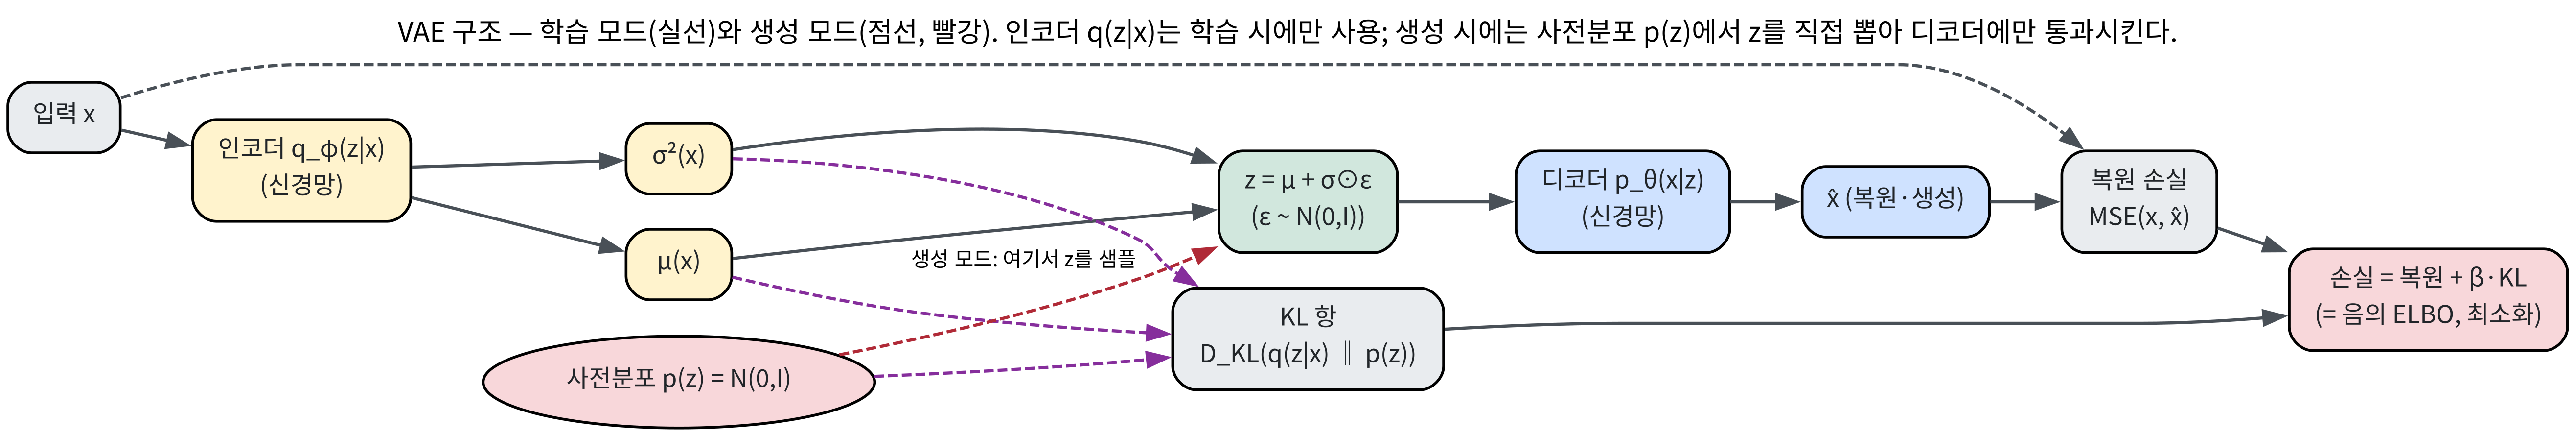
\includegraphics[width=\linewidth]{ch15_2_vae_structure.png}
      \vskip0.3em
      {\footnotesize 점선 = 생성 시 흐름(인코더 미사용), 실선 = 학습 시
      흐름}
    \end{column}
  \end{columns}
  \vskip0.5em
  \begin{block}{``매끄럽게 펼쳐놓았다''의 실체}
    학습의 \textbf{전부} = 디코더가 ``표준정규분포의 $z$''라는 입력만으로
    그럴듯한 $x$를 만들어내도록 만드는 것.
  \end{block}
\end{frame}

\begin{frame}{우도 기반 접근과 ``적분'' 문제}
  \begin{itemize}
    \item VAE는 생성형 모델 방식 중 첫 번째 — \kb{우도 기반}
      (likelihood-based): 모델이 학습 데이터를 만들어낼 확률 $P(x)$를
      (근사치로라도) \textbf{최대화}
    \item 문제:
    \[p_\theta(x) = \int p_\theta(x|z)\,p(z)\,dz\]
      가능한 모든 $z$에 대한 \textbf{적분}이라 일반적으로 계산
      불가능(intractable)
  \end{itemize}
  \vskip0.8em
  \begin{columns}[T]
    \begin{column}{0.5\textwidth}
      \textbf{GMM과의 대조 (1)}
      \begin{itemize}
        \item GMM: $p(x) = \sum_k \pi_k \mathcal{N}(x;\mu_k,\sigma_k^2)$
        \item $z$가 \textbf{유한} → 유한 합, 각 항이 정규 밀도로
          \textbf{닫힘} → 우도 정확히 계산 가능
        \item VAE: $z$가 \textbf{연속} → 적분으로 바뀜, 디코더가 신경망
         이라 닫힌 형태 없음
      \end{itemize}
    \end{column}
    \begin{column}{0.5\textwidth}
      \textbf{GMM과의 대조 (2)}
      \begin{itemize}
        \item GMM: 이산이라 사후확률(책임값) 계산 가능 → \kb{EM} 성립
        \item VAE: 이 적분의 ``역방향'' $p(z|x)$도 계산 불가능 →
          \textbf{E-step 수행 불가}
        \item 그래서 E-step을 신경망 $q_\phi(z|x)$로 \textbf{대체}(근사)
      \end{itemize}
    \end{column}
  \end{columns}
\end{frame}

\begin{frame}{ELBO: 계산 가능한 하한으로 우회}
  직접 계산할 수 없는 $\log p_\theta(x)$ 대신, 다음이 성립함을 보일 수
  있다:
  \[
  \log p_\theta(x) \ge
  \mathbb{E}_{z \sim q_\phi(z|x)}[\log p_\theta(x|z)]
  - D_{KL}\big(q_\phi(z|x) \,\|\, p(z)\big)
  \]
  우변을 \kb{ELBO}(Evidence Lower BOund)라 부른다. 두 항의 의미:
  \vskip0.6em
  \begin{block}{첫 항: 복원 항}
    $\mathbb{E}[\log p_\theta(x|z)]$ — 인코더가 만든 $z$로 디코더가
    원본 $x$를 얼마나 잘 복원하는가 (일반 오토인코더의 복원 오차와
    본질적으로 같음).
  \end{block}
  \vskip0.4em
  \begin{block}{둘째 항: 정규화 항}
    $D_{KL}(q_\phi(z|x) \| p(z))$ — 인코더 분포가 목표 사전분포 $p(z)$
    (보통 표준정규)에서 얼마나 벗어났는가 (KL divergence, Ch.\,2.3
    섀넌의 정보이론에서 소개). 이 항이 바로 잠재 공간을 매끄럽게
    만드는 힘.
  \end{block}
\end{frame}

\begin{frame}{ELBO 유도: 옌센 부등식 한 번}
  \textbf{``왜 $\log p(x)$는 ELBO보다 항상 큰가?''}를 직접 확인.
  $q$를 \textbf{우리가 고르는} 임의의 근사분포로 놓고
  $p(x) = \int p(x,z)\,dz$에 $\frac{q(z)}{q(z)}$($=1$)을 끼워넣는다:
  \[
  \log p(x) = \log \int q(z)\,\frac{p(x,z)}{q(z)}\,dz
  = \log \mathbb{E}_{z \sim q}\left[\frac{p(x,z)}{q(z)}\right]
  \]
  $\log$가 \textbf{오목함수}이므로 \kb{옌센 부등식}
  ($\log \mathbb{E}[X] \ge \mathbb{E}[\log X]$, Ch.\,2.3 교차 엔트로피
  부등식과 같은 근원)을 적용:
  \[
  \log p(x) \ge \mathbb{E}_q\left[\log \frac{p(x,z)}{q(z)}\right]
  = \underbrace{\mathbb{E}_q[\log p(x|z)]}_{\text{복원 항}}
  - \underbrace{D_{KL}(q \| p)}_{\text{정규화 항}}
  \]
  마지막 등호에서 $\mathbb{E}_q[\log p(z)] - \mathbb{E}_q[\log q(z)]
  = -D_{KL}(q\|p)$를 썼다. \textbf{옌센 부등식 한 번이 전부}다.
\end{frame}

\begin{frame}{갭의 정체: ELBO 최대화 = 변분 베이즈}
  \begin{itemize}
    \item 부등식의 ``갭'' $p(x) - \text{ELBO}$는 사실
      \textbf{$D_{KL}(q \| p(z|x))$} — 근사분포가 \textbf{진짜
      사후분포}와 얼마나 다른가
    \item $\Rightarrow$ ELBO를 최대화하는 것은 \textbf{사후분포 근사
      $q$를 정확히 만드는 것}과 동치
    \item ``ELBO 최대화 = \kb{변분 베이즈}''라는 말이 정확히 이 뜻
    \item 등호가 성립하는 조건: $p(x,z)/q(z)$가 $z$에 대해 상수,
      즉 \textbf{$q(z) = p(z|x)$}일 때 (15.1절 연습문제 5 폴백 버전의
      바로 그 조건)
  \end{itemize}
  \vskip0.8em
  \begin{block}{학습에서의 의미}
    $\log p_\theta(x) \ge \text{ELBO}$이므로, \textbf{ELBO를 최대화하면
    실제 우도의 하한도 함께 올라감} — 직접 계산 못 하는 목표를
    계산 가능한 \textbf{대리(surrogate)} 목표로 바꿔치기한 것.
  \end{block}
\end{frame}

\begin{frame}{손으로 한 번: 1차원 장난감에서 ELBO}
  15.1절 GMM과 같은 모양(1 근처·9 근처 두 봉우리)의 데이터.
  1차원 $z$, 디코더 $p(x|z) = \mathcal{N}(x; z, 1)$, 사전
  $p(z) = \mathcal{N}(0,1)$. 근사분포를 \textbf{아무렇게나}
  $q(z) = \mathcal{N}(1,1)$으로 고르고 $x = 1$에 대해 ELBO를 계산:
  \vskip0.6em
  \begin{itemize}
    \item \textbf{복원 항}:
      $\mathbb{E}_{z\sim\mathcal{N}(1,1)}[\log \mathcal{N}(x; z, 1)]$
      \item $z$가 평균 1·분산 1이면 $\mathbb{E}[(x-z)^2] = (x-1)^2 + 1$
      (분산 $\sigma_z^2$ 항 — 아래 ``자주 하는 실수'' ① 참고)
    \item $\Rightarrow -\frac{1}{2}[(x-1)^2 + 1 + \log 2\pi]
      \approx -\frac{1}{2}[0 + 1 + 1.838] = \mathbf{-1.419}$
    \item \textbf{정규화 항}:
      $D_{KL}(\mathcal{N}(1,1) \| \mathcal{N}(0,1))$ — 정규분포 사이 KL은
      닫힌 형태:
      $\frac{1}{2}(\sigma_q^2 + \mu_q^2 - 1 - \log \sigma_q^2)
      = \frac{1}{2}(1 + 1 - 1 - 0) = \mathbf{0.5}$
    \item \textbf{ELBO} $= -1.419 - 0.5 = \mathbf{-1.919}$
  \end{itemize}
\end{frame}

\begin{frame}{진짜 $\log p(x)$와 비교: 부등식이 실제로 성립}
  \begin{itemize}
    \item \textbf{진짜} $\log p(1)$: $p(x) = \int \mathcal{N}(x|z,1)\,
      \mathcal{N}(z;0,1)\,dz$ — ``정규분포 두개의 합(적분)은
      정규분포'' → $\mathcal{N}(x; 0, 2)$
    \item $\log p(1) = -\frac{1}{4} - \frac{1}{2}\log(4\pi)
      \approx \mathbf{-1.516}$
    \item \kq{부등식이 실제로 성립: $-1.516 \ge -1.919$}
    \item 갭 $-1.516 - (-1.919) = 0.403$은 정확히
      $D_{KL}(q \| p(z|x))$ — 진짜 사후
      $p(z|x) = \mathcal{N}(0.5, 0.5)$ (Ch.\,3 GDA 공식: 두 정규분포의
      ``합''이 사후)과 엉터리 근사 $\mathcal{N}(1,1)$ 사이의 거리
  \end{itemize}
  \vskip0.8em
  \begin{block}{$x = 9$로 다시 계산}
    복원 항 $\approx -33.419$, 정규화 항 0.5 → ELBO $\approx -33.92$.
    진짜 $\log p(9) = \log \mathcal{N}(9;0,2) \approx -21.52$ —
    \textbf{갭이 12.40으로 벌어짐}. $q = \mathcal{N}(1,1)$은 $x=1$
    근처에선 ``그럭저럭'' 근사(갭 0.4)지만 $x=9$엔 \textbf{완전히
    부적합}(갭 12.4).
  \end{block}
\end{frame}

\begin{frame}{숫자가 말하는 것: 입력별 분포가 필요한 이유}
  \begin{itemize}
    \item ``어느 쪽 봉우리에도 속하지 않는'' $x = 5$의 우도도 낮음:
      $\log p(5) = \log \mathcal{N}(5;0,2) \approx -7.52$
      ($x=1$의 $-1.52$보다 훨씬 낮음)
    \item $\Rightarrow$ 근사분포가 \textbf{데이터마다} 얼마나 잘
      맞아야 하는지
  \end{itemize}
  \vskip0.8em
  \begin{block}{ELBO를 최대화하는 것은 ``근사분포를 잘 고르는 것''}
    실제 학습에서는 $q$를 \textbf{$x$마다 다른} (인코더가 만들어내는)
    $q_\phi(\cdot|x)$로 놓아, \textbf{복원 항이 좋아질수록 정규화 항이
    나빠지는(또는 그 반대)} \textbf{균형}이 학습이 끝난 지점에서
    결정된다. 그 균형이 실제로 어디에 잡히는지 다음 실습에서 확인.
  \end{block}
\end{frame}

\begin{frame}[fragile]{VAE 손실함수: ELBO의 코드}
\begin{lstlisting}
def vae_loss(x, x_reconstructed, mu, log_var):
    # 복원 손실 (여기서는 MSE로 근사)
    recon_loss = sum((x[i] - x_reconstructed[i]) ** 2 for i in range(len(x)))
    # KL divergence: 정규분포 q(mu, sigma^2)와 표준정규 N(0,1)의 닫힌 형태
    kl_loss = -0.5 * sum(1 + log_var[i] - mu[i]**2 - math.exp(log_var[i])
                          for i in range(len(mu)))
    return recon_loss + kl_loss  # ELBO 최대화 = 음의 ELBO 최소화
\end{lstlisting}
  \vskip0.4em
  정규분포 $\mathcal{N}(\mu, \sigma^2)$와 표준정규 $\mathcal{N}(0,1)$
  사이의 KL은 닫힌 형태:
  \[D_{KL}\big(\mathcal{N}(\mu, \sigma^2) \,\|\, \mathcal{N}(0,1)\big)
  = \frac{1}{2}\left(\sigma^2 + \mu^2 - 1 - \log \sigma^2\right)\]
  \vskip0.3em
  {\footnotesize 코드에서 이 값을 \textbf{음수}로 쓰는 이유:
  $-\frac{1}{2}(\sigma^2 + \mu^2 - 1 - \log\sigma^2)$는 ELBO 정규화 항에
  마이너스가 붙은 형태($-D_{KL}$)이며, 복원 항과 더하면 ELBO 그
  자체. 손실 = \textbf{음의 ELBO}를 최소화.}
\end{frame}

\begin{frame}{Reparameterization Trick}
  \begin{itemize}
    \item $z$를 확률분포에서 \textbf{직접 샘플링}하면 ``샘플링''
      연산은 \textbf{미분이 안 됨} → 역전파가 인코더까지
      흘러가지 못함
    \item \kb{Reparameterization Trick} (Rezende et al., 2014):
    \[z = \mu + \sigma \odot \epsilon, \qquad
      \epsilon \sim \mathcal{N}(0,1)\]
    \item $\epsilon$은 \textbf{무작위성을 밖으로 빼낸 상수 취급}
    \item $\mu, \sigma$로 가는 경로가 전부 미분 가능한 연산(곱셈,
      덧셈) → 역전파가 인코더 파라미터까지 정상적으로 흐름
  \end{itemize}
  \vskip0.8em
  \begin{block}{왜 꼭 필요한가 (Ch.\,9 연결)}
    역전파는 연쇄법칙으로 미분 가능한 연산 사슬을 거슬러 올라가는
    것 — ``확률분포에서 무작위 추출'' 연산은 미분이 정의되지 않는다.
    이 트릭이 없으면 VAE의 인코더를 학습할 수 없다.
  \end{block}
\end{frame}

\begin{frame}[fragile]{실습: 두 봉우리 데이터로 작은 VAE}
  15.1절 GMM 예제와 같은 모양(1 근처·9 근처 두 봉우리)의 1차원 데이터로
  실제 VAE를 학습:
\begin{lstlisting}
import torch, torch.nn as nn

class VAE(nn.Module):
    def __init__(self, latent_dim=2):
        super().__init__()
        self.enc = nn.Sequential(nn.Linear(1, 16), nn.ReLU())
        self.mu = nn.Linear(16, latent_dim)
        self.logvar = nn.Linear(16, latent_dim)
        self.dec = nn.Sequential(nn.Linear(latent_dim, 16), nn.ReLU(), nn.Linear(16, 1))
    def forward(self, x):
        h = self.enc(x)
        mu, logvar = self.mu(h), self.logvar(h)
        z = mu + torch.exp(0.5*logvar) * torch.randn_like(mu)  # reparameterization trick
        return self.dec(z), mu, logvar
\end{lstlisting}
\end{frame}

\begin{frame}{학습 곡선: 두 항의 줄다리기}
  500 에폭 학습 후 (스크래치패드 실행 검증):
  \begin{center}\small
  \begin{tabular}{@{}ll@{}}
    \toprule
    에폭 & loss (복원 손실, KL) \\
    \midrule
    0   & 57.381 (54.392, 2.989) \\
    100 & 3.051  (0.852,  2.199) \\
    499 & 2.063  (0.482,  1.581) \\
    \bottomrule
  \end{tabular}
  \end{center}
  \vskip0.5em
  \begin{itemize}
    \item 손실이 57.4 $\to$ 2.06까지 꾸준히 감소 (무작위 초기화에 따라
      수치 변동 — 시드 42 고정 시 epoch 0: 36.737, epoch 499: 1.667)
    \item 복원 손실이 에폭 99(0.428)보다 에폭 499(0.438)에서 \textbf{아주
      약간 오르는} 구간 존재
    \item ``총 손실 감소'' $\neq$ ``복원 손실만 감소'' — KL 항이 크게
      줄어드는 동안 복원 손실이 아주 약간 오르는 것이 두 항의
      \textbf{균형이 다시 짜여지는} 과정 (epoch 199에서 복원 손실 0.461로
      더 크게 올랐다가 다시 내려옴)
  \end{itemize}
\end{frame}

\begin{frame}{인코더가 두 봉우리에 배운 분포}
  학습이 끝난 뒤 인코더가 두 봉우리 각각에 어떤 분포를 배웠는지
  확인 (시드 42 실행):
  \begin{itemize}
    \item 왼쪽 봉우리($\approx 1$)의 점들:
      평균 $(\mu_1, \mu_2) \approx (0.5, -0.88)$
    \item 오른쪽($\approx 9$): $(-0.77, 1.42)$ 근처로 \textbf{분리}
    \item 분산은 아주 작음 ($\log\sigma^2 \approx -1.7$ 이하)
  \end{itemize}
  \vskip0.6em
  \begin{block}{GMM과의 연결}
    인코더가 ``왼쪽 점''과 ``오른쪽 점''을 잠재 공간에서
    \textbf{다른 위치에, 좁은 분포로} 배치 — GMM의 이산적 클러스터
    할당에 해당하는 \textbf{연속적(soft) 버전}.
  \end{block}
  \vskip0.4em
  {\footnotesize 두 군집의 분산도 작게 수렴 — ``여기''에 속한 점은
  거의 결정적으로 배정되는, GMM의 책임값이 사실상 0/1에 가까워진
  것과 같은 상태. 그 위치가 \textbf{원점(사전분포의 중심)을 사이에
  두고} 대략 대칭 — KL 항이 두 군집을 원점 쪽으로 끌어당긴 흔적.}
\end{frame}

\begin{frame}{생성 모드: 원본을 전혀 보지 않고}
  학습이 끝난 뒤 \textbf{원본 데이터를 전혀 보지 않고},
  표준정규분포 $\mathcal{N}(0,1)$에서 $z$를 1000개 무작위 추출 →
  \textbf{디코더에만} 통과:
  \begin{center}\small
  \begin{tabular}{@{}l@{}}
    \toprule
    생성된 샘플: 평균 4.83, 표준편차 3.84 \\
    1(왼쪽 봉우리) 근처 비율: 59.1\%, \; 9(오른쪽 봉우리) 근처 비율: 40.9\% \\
    \bottomrule
  \end{tabular}
  \end{center}
  \vskip0.5em
  \begin{itemize}
    \item 원본이 두 봉우리에 대략 절반씩인데, 디코더가 잠재 공간의
      표준정규 $z$만으로 그 두 봉우리를 \textbf{대략 6:4로 재현}
    \item 완벽하진 않지만 — ``인코더가 데이터를 잠재 공간에 매끄럽게
      펼쳐놓고, 어디서 샘플링해도 그럴듯한 데이터가 나온다''는
      설계 목표가 실제로 작동하는 것을 확인
    \item (시드 42 실행: 평균 3.40·표준편차 2.82, 비율 74.9:25.1로 더
      기울어짐 — 인코더가 두 봉우리를 정확히 \textbf{대칭적으로 배치하지
      못해서}. 시드를 바꾸면 비율이 바뀌지만 큰 그림에는 영향 없음)
  \end{itemize}
\end{frame}

\begin{frame}{학습 과정 2$\times$2 시각화}
  \begin{columns}[T]
    \begin{column}{0.45\textwidth}
      \centering
      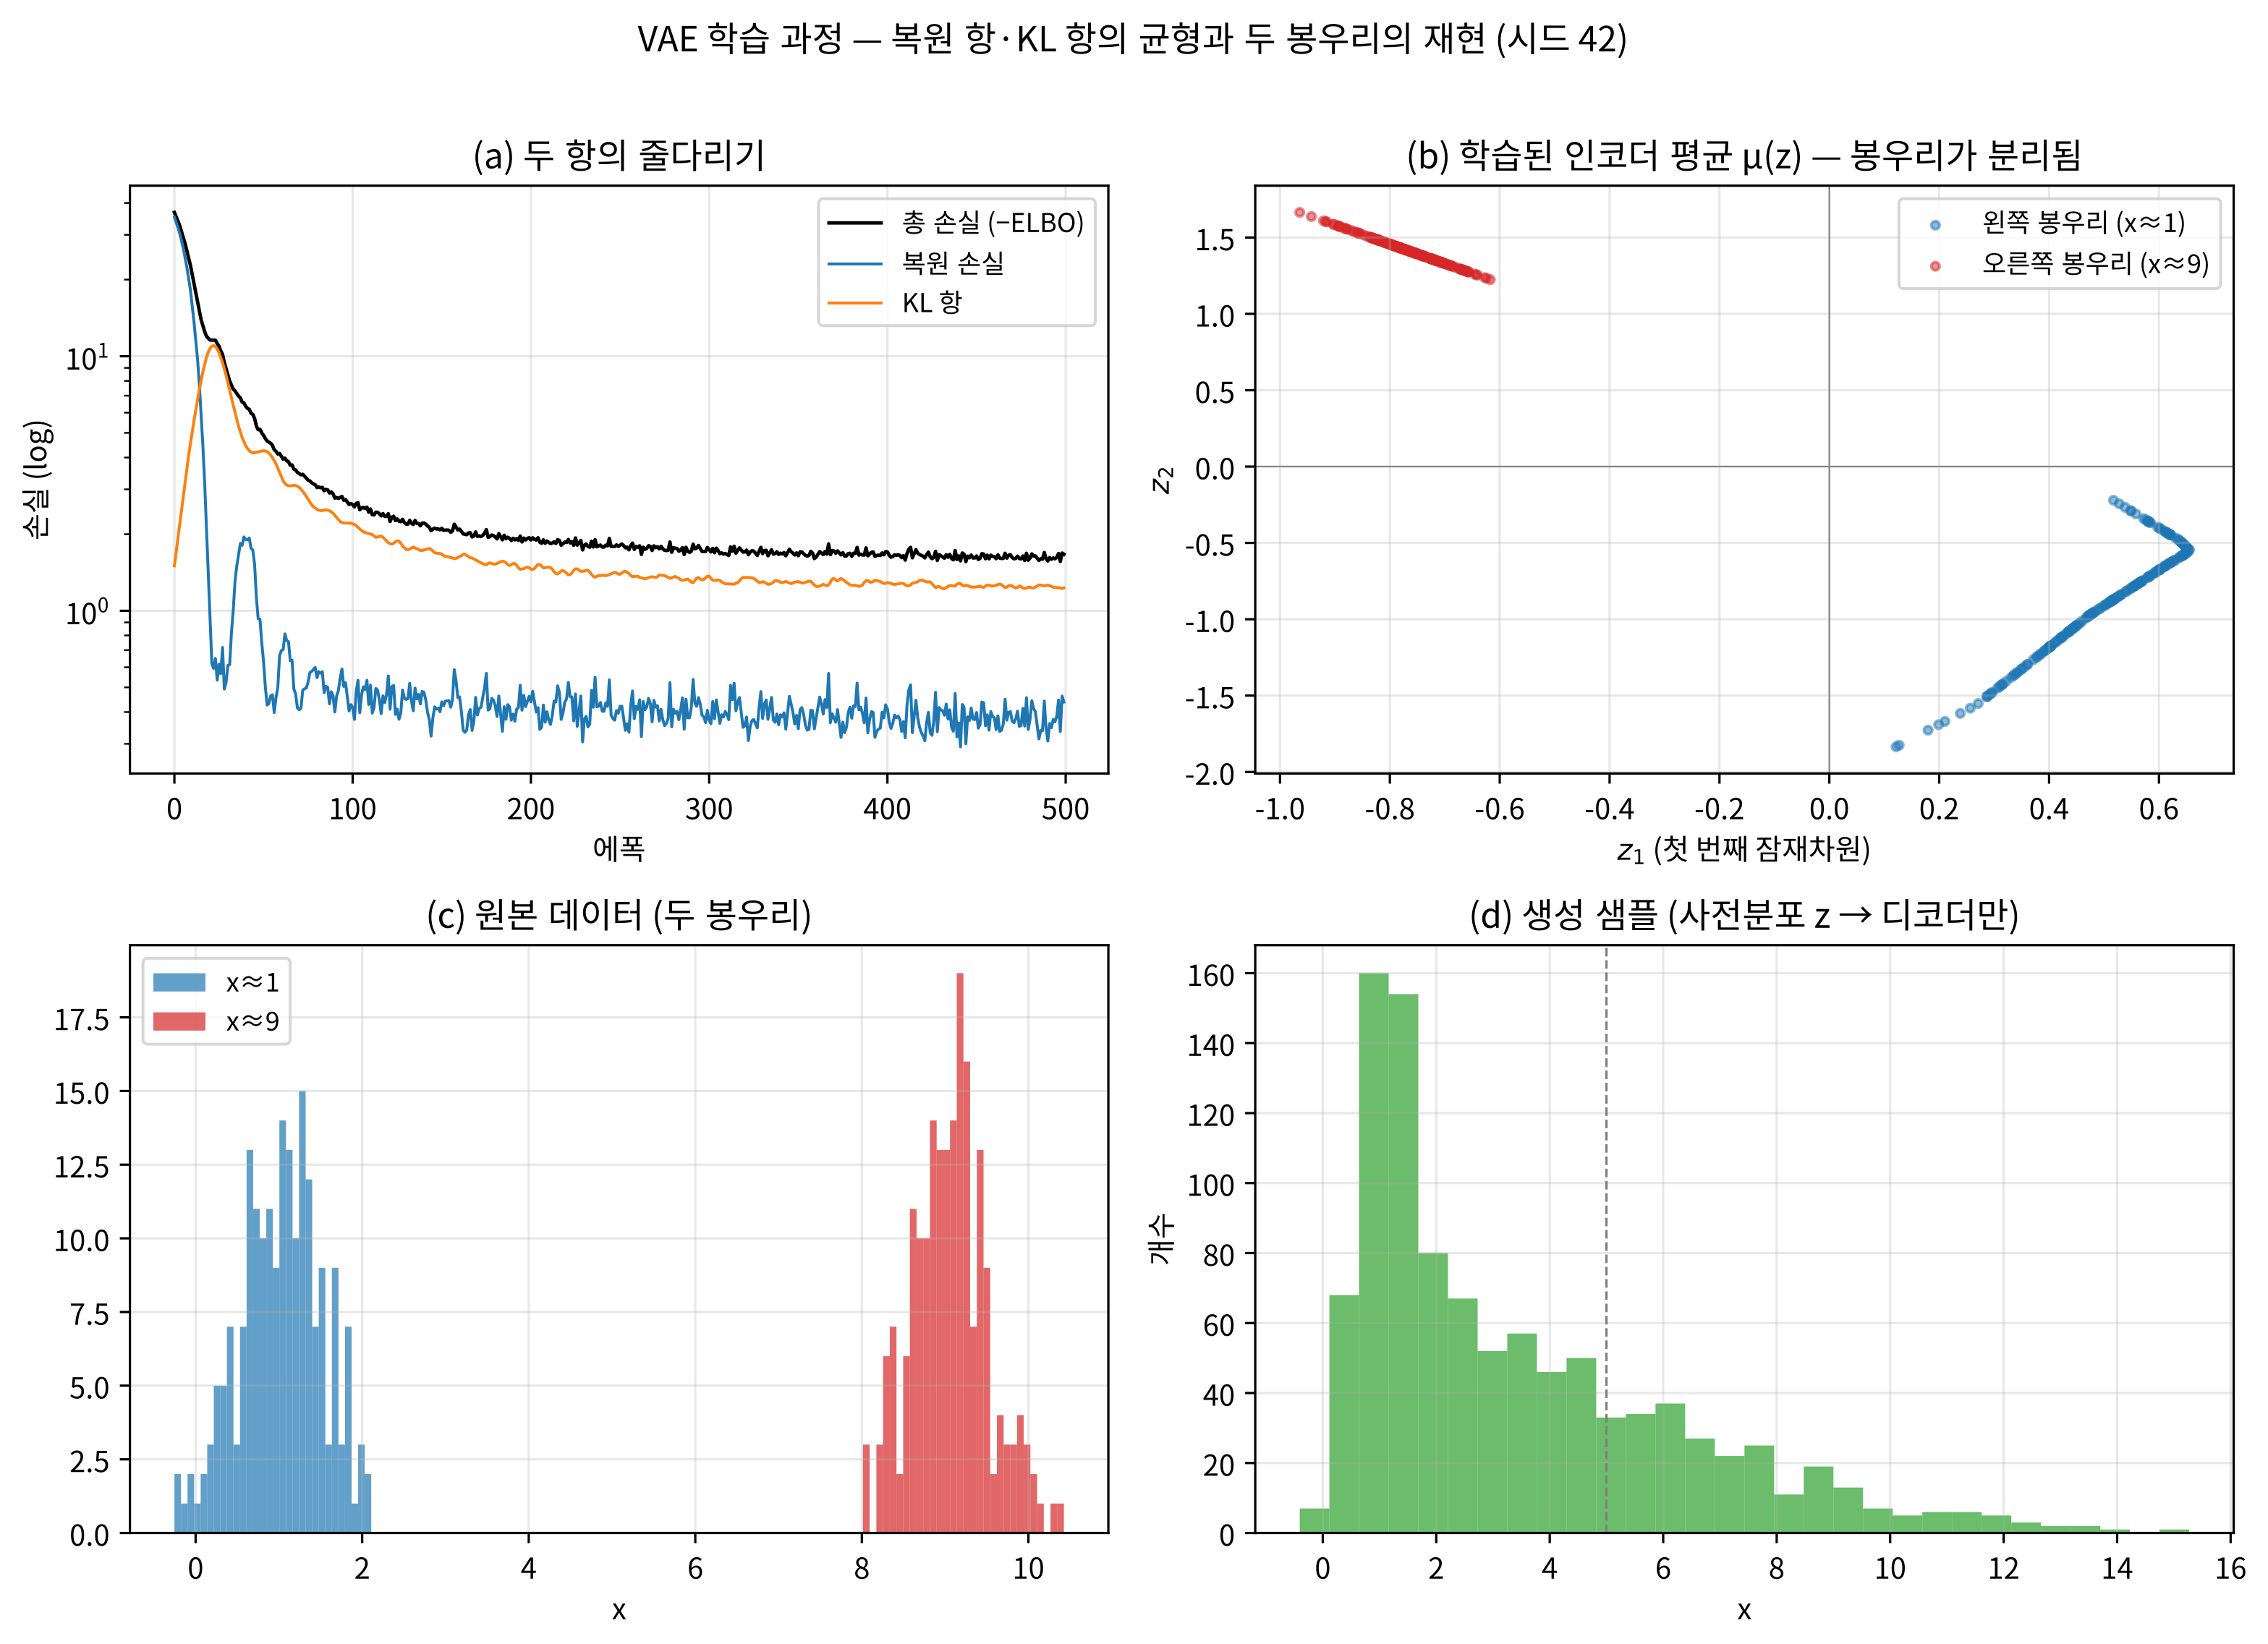
\includegraphics[width=\linewidth]{ch15_2_vae_elbo.png}
      \vskip0.3em
      {\footnotesize (a) 손실 곡선 (log) (b) 인코더가 매긴 $\mu(z)$
      (c) 원본 (d) 생성 샘플}
    \end{column}
    \begin{column}{0.53\textwidth}
      \small
      \begin{itemize}
        \item \textbf{(a)}: KL 항이 2.2에서 1.2로 \textbf{큰 폭으로
          떨어짐}, 복원 손실은 0.43 부근에서 \textbf{거의 제자리}
          — 두 항이 서로 ``견제''하며 균형으로 수렴
        \item \textbf{(b)}: GMM의 이산적 클러스터 할당의
          \textbf{연속적(soft) 버전} — 각 점에 매긴 평균이
          ``왼쪽 $\approx (0.5,-0.9)$'', ``오른쪽 $\approx (-0.8,1.4)$''
          근처의 \textbf{좁은 군집}으로 모임
        \item \textbf{(c)(d)}: 생성 샘플(1000개)이 두 봉우리를
          히스토그램으로 대략 재현
      \end{itemize}
    \end{column}
  \end{columns}
\end{frame}

\begin{frame}{$\beta$-VAE: 두 항의 균형점을 ``학습률처럼''}
  복원 항과 정규화 항의 계수를 1:1로 고정한 것은 하나의 선택일 뿐.
  $\beta$-VAE (H. Kingma, Salimans, Welling, 2016)는 정규화 항에
  계수 $\beta$를 붙여 $\mathcal{L} = \mathbb{E}[\log p(x|z)]
  - \beta\, D_{KL}$로 일반화:
  \vskip0.6em
  \small
  \begin{tabular}{@{}lrrr@{}}
    \toprule
    $\beta$ & 복원 손실 & KL & 생성 샘플 표준편차 \\
    \midrule
    0   & 0.016 & 19.1 & 0.58 \\
    0.1 & 0.068 & 5.61 & 0.91 \\
    0.5 & 0.232 & 1.70 & 1.67 \\
    1.0 (기본) & 0.378 & 1.22 & 2.05 \\
    2.0 & 0.546 & 0.90 & 2.42 \\
    \bottomrule
  \end{tabular}
  \vskip0.8em
  \begin{itemize}
    \item $\beta = 0$: 정규화 항 \textbf{완전히 끔} → 일반 오토인코더로
      복귀. 복원 손실 0.016(아주 작음)이지만 KL 19.1(잠재 공간이
      표준정규와 거의 무관), 생성 표준편차 0.58 — \textbf{데이터(표준편차
      4.05)보다 훨씬 좁음}. 잠재 공간이 ``여기저기 흩어져 있어 아무 데서
      샘플링해도 안 된다''는 원래 문제 그대로.
    \item $\beta = 2$: 정규화 항 강화 → KL 0.90으로 작아지지만 복원
      손실 0.55로 올라가고, 생성 표준편차 2.42 — \textbf{정보를 더
      압축}하는 대가로 복원 품질이 약간 떨어짐.
  \end{itemize}
  \vskip0.4em
  {\footnotesize $\beta$는 ``복원 품질 vs 잠재 공간의 매끄러움(정규성)''을
  \textbf{학습률처럼 튜닝하는 하이퍼파라미터}. (``VAE가 왜 흐릿한지''의
  답변도 결국 이 $\beta$의 균형 문제에서 출발.)}
\end{frame}

\begin{frame}{자주 하는 실수 ①②: KL 항 계산}
  \begin{block}{① 복원 항 기대값에 $\sigma^2$ 항을 빼먹는 것}
    $\mathbb{E}[\log p(x|z)]$를 계산할 때 $(x-\mu)^2$만 쓰고 분산
    $\sigma_q^2$ 항을 빼먹으면 복원 항이 $-0.919$로 \textbf{과소평가}
    (정답 $-1.419$). $z = \mu + \sigma\epsilon$일 때 $\mathbb{E}[(x-z)^2]
    = (x-\mu)^2 + \sigma^2$ — ``평균으로 대체''한 것만으로 오차가
    사라지지 않음. $\sigma^2$가 큰(인코더가 불확실한) 입력에서 손실값이
    실제보다 크게 나타나는(= ELBO 과소평가) 방향으로 오류를 만들어,
    ``정규화 항을 줄이는데 왜 손실이 안 줄지''를 진단할 때 혼란의 원인.
  \end{block}
  \vskip0.4em
  \begin{block}{② KL 항을 ``분산만'' 계산하는 것}
    인코더가 $(\mu, \sigma^2)$를 함께 내놓는데, KL 항에 $\mu^2$(위치)
    항을 빼먹고 $\sigma^2 - 1 - \log\sigma^2$만 쓰면, \textbf{$\mu$에
    대한 그래디언트가 0} — 인코더의 평균 출력 위치에 대해 정규화 항이
    아무 작용도 하지 않아 ``분산만 조절된다''는, 학습이 이상하게
    멈추는 원인. $\frac{1}{2}(\sigma^2 + \mu^2 - 1 - \log\sigma^2)$의
    $\mu^2$ 항이 \textbf{인코더의 위치($\mu$)를 원점 방향으로
    끌어당기는 힘}임을 꼭 기억.
  \end{block}
\end{frame}

\begin{frame}{자주 하는 실수 ③④⑤}
  \begin{itemize}
    \item \kb{③ $\beta$를 너무 크게 올려 ``정규화만'' 보는 학습} —
      $\beta$-VAE에서 $\beta$를 극단적으로 올리면 KL이 0에 가까워지고
      복원 손실은 커짐 — ``인코더가 데이터를 전혀 담지 않고
      표준정규분포를 그대로 뱉는'' 방향으로 \textbf{치팅}할 유인이
      강해짐. $\beta = 2$ 이미 복원 손실 0.55(기본 1.0 대비 1.45배).
      ``KL을 많이 줄이면 잠재 공간이 더 매끄러우니 좋다''는 생각은
      $\beta$-VAE의 \textbf{균형을 무너뜨리는} 것.
    \item \kb{④ 생성 샘플을 ``인코더''에 다시 넣는 것} — 생성 모드에서는
      사전분포 $p(z)$에서 $z$를 뽑아 \textbf{디코더에만} 통과. 인코더를
      다시 거치면 ``학습 데이터에 가까운 $z$''만 만들어져 ``새로운
      샘플''이 안 나옴 (인코더는 생성 시 \textbf{사용하지 않는} 것이
      VAE의 구조 — 구조도의 점선/실선 구분이 말해줌).
    \item \kb{⑤ ``ELBO가 높으면 진짜 우도도 반드시 높다''는 착각} —
      ELBO는 \textbf{하한}이지 근사가 아님. $q$가 진짜 사후
      $p(z|x)$와 크게 다르면 갭이 커짐 ($x = 9$ 예제: 갭 12.4,
      진짜 $-21.5$, ELBO $-33.9$). ``ELBO 높음 $\to$ 우도 높음''은
      \textbf{항상} 성립(하한이니까), ``ELBO 낮음 $\to$ 우도 낮음''은
      \textbf{반드시} 성립하지 않음 ($q$가 나쁘면 갭이 큼).
  \end{itemize}
\end{frame}

\begin{frame}{확인 문제 (15.1)}
  \begin{enumerate}
    \item \textbf{ELBO 부등식의 갭.} $\log p(x) - \text{ELBO} =
      D_{KL}(q \| p(z|x))$임을 유도한 뒤, $q = p(z|x)$일 때만 갭이 0이
      된다는 것을 한 문장으로 설명.
    \item \textbf{정규분포 합 = 정규분포.}
      $\mathcal{N}(x; z,1) \cdot \mathcal{N}(z;0,1)$에 대해 $z$로 적분
      하면 $\mathcal{N}(x; 0, 2)$가 된다는 것을, ``두 독립 정규분포의
      합은 정규분포''라는 사실로부터 한 문장으로 설명.
    \item \textbf{손계산 재현.} $x = 9$ 예제에서 복원 항이
      $\approx -33.4$가 되는 것을 직접 계산 (힌트: $(x-\mu)^2 = 64$,
      $\sigma_q^2 = 1$, $\log 2\pi \approx 1.838$ 대입).
  \end{enumerate}
  \vskip0.8em
  \begin{block}{핵심 요약}
    ELBO = \textbf{복원 항} $-$ \textbf{KL 정규화 항}.
    \textbf{ELBO 최대화 = 사후분포 근사 $q$를 정확히 만드는 것
    (변분 베이즈)}. \; $\mu^2$ 항은 \textbf{위치를 원점 쪽으로
    끌어당기는 힘}, $\sigma^2$ 항은 \textbf{너비를 제어}.
  \end{block}
\end{frame}

\begin{frame}{자주 묻는 질문: 두 항 중 하나만 최적화하면?}
  \begin{itemize}
    \item \textbf{복원 항만}(KL 없이): 일반 오토인코더와 같아져
      잠재 공간이 매끄럽지 않아 샘플링 품질이 나빠짐 — 실습에서
      KL 항이 없었다면 생성 샘플이 두 봉우리를 재현하지 못했을
      가능성 큼
    \item \textbf{KL 항만}(복원 없이): 인코더가 아무 정보도 담지 않고
      그냥 표준정규분포를 그대로 뱉는 방향으로 ``치팅'' — 복원이
      전혀 안 되는 무의미한 모델
    \item $\Rightarrow$ \kq{두 항의 \textbf{균형}이 VAE의 핵심}
  \end{itemize}
\end{frame}

\begin{frame}{자주 묻는 질문: 리파라미터화 · 흐릿함}
  \begin{block}{Reparameterization trick이 왜 꼭 필요한가?}
    Ch.\,9: 역전파는 연쇄법칙으로 미분 가능한 연산 사슬을 거슬러
    올라가는 것. ``확률분포에서 무작위 추출'' 연산은 미분이 정의
    안 됨. $z = \mu + \sigma \odot \epsilon$으로 다시 쓰면 무작위성은
    $\epsilon$(입력과 무관한 상수)에만, $\mu, \sigma$로 가는 경로는
    전부 미분 가능(곱셈·덧셈) → 역전파가 인코더 파라미터까지
    정상적으로 흐름.
  \end{block}
  \vskip0.4em
  \begin{block}{KL 항이 ``흐릿함''의 원인이라는 말은?}
    복원 항은 \textbf{기대값} $\mathbb{E}_{z\sim q}[\log p(x|z)]$를
    최적화 — 인코더 분포의 \textbf{모든} $z$로 복원했을 때의
    \textbf{평균}이 좋아야 함. 분포가 넓을수록($\sigma^2$ 클수록)
    복원된 $x$ 후보가 넓게 퍼져 ``모든 $z$의 평균''이 흐려짐 →
    VAE 생성 이미지의 \textbf{흐릿함(blurry)} 근원. $\beta$를 크게
    하면 더 강해짐 (정보를 더 압축하니까). GAN이 ``한 개 $z$ → 한 개
    $x$''를 \textbf{결정적으로} 학습(흐릿하지 않은 선명함)하는 이유도
    결국 ``기대값 최적화 vs 결정적 복원''의 차이.
  \end{block}
\end{frame}

\begin{frame}{자주 묻는 질문: EM/GMM과의 관계 · 차원 선택}
  \begin{block}{VAE와 15.1절 EM/GMM의 관계?}
    GMM: $z$가 \textbf{이산}(클러스터 번호)이라 E-step(책임값)이 닫혀
    계산 가능 → EM 성립. VAE: $z$가 \textbf{연속}이라 E-step 자체가
    계산 불가능 → \textbf{E-step을 신경망 $q_\phi(z|x)$로 대체}(근사),
    M-step을 \textbf{역전파}로 수행. ``EM의 E-step을 신경망이
    대신한다''. M-step도 ``잠재변수별 파라미터 가중평균''이 아니라
    ``전체 파라미터를 ELBO의 그래디언트로 갱신''으로 바뀜.
  \end{block}
  \vskip0.4em
  \begin{block}{$\texttt{latent\_dim} = 2$가 왜 2차원인가?}
    \textbf{학습 대상이 아니라 하이퍼파라미터}. 두 봉우리 데이터:
    ``두 가지 원인''이 있어 1차원으로 충분, 2차원이면 두 봉우리가
    원점 중심의 \textbf{대칭} 위치로 자연스럽게 배치. 이미지 데이터:
    20$\sim$200 차원이 흔함 — 너무 작으면 복원 품질 떨어짐, 너무
    크면 ``사용하지 않는 차원''으로 가득 차 KL이 커짐.
  \end{block}
\end{frame}

\section{15.2 GAN, Diffusion, 그리고 세 원리 비교}

\begin{frame}{15.1의 다음: 우도 기반과 확연히 다른 두 방식}
  \begin{itemize}
    \item 15.1절 \kb{VAE} = 4.4절 GMM/EM이 던진 질문을 신경망으로
      근사 — 풀리지 않는 E-step을 인코더로 대체, 우도의 하한(ELBO)을
      역전파로 최대화하는 \textbf{우도 기반}의 마지막 방식
    \item 이번 절: 우도 기반과 \textbf{확연히 다른} 두 방식
    \item \kb{GAN}: 두 신경망의 \textbf{경쟁 게임}으로 학습
    \item \kb{Diffusion}: 노이즈를 \textbf{한 단계씩 되돌리는
      회귀 문제}로 학습
    \item 세 방식(VAE·GAN·Diffusion)이 나란히 놓이면 Chapter 15 전체의
      그림이 완성
  \end{itemize}
\end{frame}

\begin{frame}{GAN: 생성자와 판별자의 min-max 게임}
  \begin{itemize}
    \item 2014년, 몬트리올 대학교 얀 르쿤·요슈아 벵기오 연구소 박사
      과정 \kb{이언 굿펠로우(Ian Goodfellow)}: ``진짜 같은 가짜를
      만드는 모델 학습'' 대신 \textbf{두 신경망이 서로 경쟁}하게 하면?
    \item \textbf{위조범}(생성자 $G$): 가짜를 만듦
    \item \textbf{감정사}(판별자 $D$): 진짜/가짜를 구별
    \item VAE가 ``우도 최대화''라는 명확한 \textbf{단일} 목표함수가
      있었던 것과 달리, GAN은 두 네트워크가 \textbf{서로 다른,
      심지어 반대되는} 목표를 갖고 동시에 학습
  \end{itemize}
  \vskip0.6em
  \begin{block}{역사적 일화}
    2015년 GAN 논문이 처음 ICLR 워크숍에 제출됐을 때 거절, 심사평
    ``\textbf{average quality}''. 2016년 ACM 튜링상 수상 연설에서
    굿펠로우가 이 일화를 직접 소개 — ``평균적''이라 거부당한 논문이
    그해 딥러닝계를 가장 뜨겁게 달군 논문이 된 아이러니.
  \end{block}
  \vskip0.3em
  \begin{center}
  
\includegraphics[width=0.6\linewidth]{ref_gan.png}
  {\footnotesize Fig.\,1: GAN 학습 시 MNIST 샘플 품질 개선 — (a)에서
  (d)로 갈수록 생성 샘플이 실제 데이터에 가까워짐}
  \end{center}
\end{frame}

\begin{frame}{생성자·판별자와 목적함수}
  \begin{itemize}
    \item \kb{생성자}(Generator) $G$: 무작위 노이즈 $z \sim p(z)$를
      입력받아 가짜 데이터 $G(z)$를 만듦
    \item \kb{판별자}(Discriminator) $D$: 데이터를 입력받아, 그것이
      \textbf{진짜일 확률} $D(x) \in [0,1]$을 출력 (Ch.\,2
      \textbf{로지스틱회귀}와 정확히 같은 형태)
  \end{itemize}
  \vskip0.8em
  \textbf{목적함수} (min-max game):
  \[
  \min_G \max_D V(D,G) =
  \mathbb{E}_{x \sim p_{\text{data}}}[\log D(x)]
  + \mathbb{E}_{z \sim p(z)}[\log(1 - D(G(z)))]
  \]
  \vskip0.6em
  \begin{center}\small
  \begin{tabular}{@{}ll@{}}
    \toprule
    판별자 손실 & $-\big(\mathbb{E}[\log D(x)] + \mathbb{E}[\log(1 - D(G(z)))]\big)$ \\
    생성자 손실 & $-\mathbb{E}[\log D(G(z))]$ (D\_fake를 1에 가깝게) \\
    \bottomrule
  \end{tabular}
  \end{center}
\end{frame}

\begin{frame}{왜 ``균형점''을 논해야 하는가}
  \begin{itemize}
    \item 두 네트워크가 \textbf{서로 반대 목표}로 동시에 학습 →
      ``학습이 끝났다''는 것이 무슨 의미인지 \textbf{다시 정의}해야 함
    \item 게임이론에서 이런 안정 상태 = \kb{내쉬 균형}(Nash
      equilibrium) — \textbf{어느 쪽도 혼자서 전략을 바꿔서 더 나아질
      수 없는 상태}
    \item 이론적으로 이 게임의 내쉬 균형은 \textbf{$D(x) = 0.5$}
      (판별자가 진짜와 가짜를 전혀 구별하지 못함)이고, $G$가 만드는
      분포가 \textbf{실제 데이터 분포와 정확히 같아지는} 지점임이
      증명되어 있음
  \end{itemize}
  \vskip0.8em
  \kq{실전 판독: 판별자 정확도 50\%가 ``목표 운영점''. 90\%+로
  치솟으면 G가 이미 학습에서 이탈한 실패 신호.}
\end{frame}

\begin{frame}{1차원 장난감: 파라미터가 딱 1개인 GAN}
  ``내쉬 균형''이 추상적으로 들리면, \textbf{파라미터가 딱 1개인}
  장난감 GAN으로 균형을 직접 계산.
  \begin{itemize}
    \item 데이터 $x \sim \mathcal{N}(0,1)$, 생성자 분포
      $p_G = \mathcal{N}(0, s^2)$
    \item \textbf{표준편차 $s$ 하나로} 가짜 분포의 ``너비''만 바꿀 수
      있는 생성자
    \item 평균은 0으로 고정 — 데이터와 가짜가 모두 0에 대칭이라
      평균 0이 당연히 최고. 게임이 ``너비 맞추기''라는 \textbf{한 가지
      문제}로 깔끔하게 축소
  \end{itemize}
  \vskip0.8em
  \begin{block}{판별자는 로지스틱회귀}
    $D$는 $x$ 위의 로지스틱회귀(Ch.\,2.3). $G$를 고정하고 $D$를
    \textbf{완전히} 최적화하면(미니배치가 아니라 전체 데이터에서
    MLE로) 해는 \textbf{닫힌 형태}:
    \[D^*(x) = \frac{p_{\text{data}}(x)}{p_{\text{data}}(x) + p_G(x)}\]
  \end{block}
\end{frame}

\begin{frame}{놀라운 닫힌 형태: JSD로 게임의 값}
  $D^*$를 목적함수에 대입하면 게임의 값이 \textbf{닫힌 형태}로
  나옴 (GAN 원논문 Theorem 7):
  \[
  V(D^*, G) = 2\,\mathrm{JSD}(p_{\text{data}} \| p_G) - \log 4
  \]
  \vskip0.6em
  \begin{block}{JSD (Jensen-Shannon Divergence)}
    KL 발산의 ``\textbf{양방향 평균}'' 버전:
    $\mathrm{JSD}(p \| q) = \frac{1}{2} D_{KL}(p \| m) + \frac{1}{2}
    D_{KL}(q \| m)$, $m = \frac{1}{2}(p + q)$.
    \; KL은 $p, q$ 순서가 바뀌면 값이 달라지는 \textbf{비대칭} 발산인데,
    JSD는 두 방향의 평균이라 \textbf{대칭}.
  \end{block}
  \vskip0.4em
  \begin{itemize}
    \item $\mathrm{JSD} \ge 0$이고 두 분포가 \textbf{정확히 같을 때만}
      0 → $V$의 최솟값은 $p_G = p_{\text{data}}$에서의 $-\log 4$
    \item $\mathrm{JSD} \le \log 2$ → 게임의 값은 항상
      $[-\log 4,\; 0)$ 안에
  \end{itemize}
\end{frame}

\begin{frame}{``게임 값을 낮추라'' = ``JSD를 줄이라''}
  \begin{block}{생성자 관점의 명령}
    ``게임 값을 낮추라''는 것은 \textbf{``가짜와 데이터 분포의 JSD를
    줄이라''}는 것과 \textbf{정확히 같은 명령} — 두 분포를 일치시키는
    것, 즉 내쉬 균형 $s^* = 1$으로 수렴.
  \end{block}
  \vskip0.6em
  \textbf{``학습 루프''를 들여다보자} — \textbf{교대 반복} (좌표별
  최적화):
  \begin{enumerate}
    \item $G$를 고정하고 $D$를 최적화 (장난감에서는 닫힌 형태 $D^*$라
      바로 점프)
    \item $D^*$를 고정하고 $G$의 파라미터 $s$를 그라디언트 스텝으로
      한 스텝 갱신
  \end{enumerate}
  \vskip0.4em
  {\footnotesize 4.4절 EM의 뼈대 (E-step: 파라미터 고정 → 잠재변수
  채우기 / M-step: 잠재변수 고정 → 파라미터 갱신)과 같은 \textbf{좌표별
  최적화} 구조가, ``잠재변수''를 ``한 네트워크''로 바뀐 형태로
  그대로.}
\end{frame}

\begin{frame}{EM과의 결정적 차이}
  \begin{columns}[T]
    \begin{column}{0.5\textwidth}
      \kb{EM}
      \begin{itemize}
        \item E-step이 \textbf{정확한} 사후확률을 채워 넣음
        \item ``우도가 매 반복 절대 줄지 않는다''는 보장이
          \textbf{증명 가능}
      \end{itemize}
    \end{column}
    \begin{column}{0.5\textwidth}
      \kb{GAN 루프}
      \begin{itemize}
        \item (1)이 일반적으로 \textbf{완전 최적화가 아닌 근사}
        \item 매 $D$ 갱신마다 $G$가 내려다보는 \textbf{경사면 자체가
          바뀌고}
        \item 게임 값에 \textbf{단조 감소 보장이 없음}
      \end{itemize}
    \end{column}
  \end{columns}
  \vskip0.8em
  \begin{block}{이 장난감이 운 좋은 이유}
    게임 값이 $s$의 매끄러운 함수로 \textbf{유일하게} 최소가 $s = 1$
    에 있어 \textbf{단조하게} 수렴. 실전 GAN의 ``나쁜 소식들''(등락,
    발산, 모드 붕괴)이 아직 안 보이는 이유 = 이 장난감에 \textbf{국소
    균형이 딱 하나}뿐. 여러 개의 국소 균형이 존재하려면, 데이터
    분포의 ``여러 모드 중 일부만 덮는'' 가짜 분포도 균형 후보가 되는
    \textbf{고차원 세계}가 필요.
  \end{block}
\end{frame}

\begin{frame}{40스텝 교대 최적화 궤적}
  $s_0 = 2.0$, 학습률 $\eta = 0.15$로 40스텝 (수반 노트북 2절):
  \vskip0.6em
  \small
  \begin{tabular}{@{}lrrr@{}}
    \toprule
    스텝 & $s$ & $V(D^*, G)$ & $D^*(0)$ \\
    \midrule
    0   & 2.000 & $-1.201$ & 0.667 \\
    10  & 1.664 & $-1.276$ & 0.625 \\
    20  & 1.339 & $-1.346$ & 0.572 \\
    30  & 1.113 & $-1.381$ & 0.527 \\
    40  & 1.026 & $-1.386$ & 0.507 \\
    $\infty$ & 1.000 & $-\log 4 \approx -1.386$ & 0.500 \\
    \bottomrule
  \end{tabular}
  \vskip0.8em
  \begin{columns}[T]
    \begin{column}{0.55\textwidth}
      \begin{itemize}
        \item \textbf{(i)} 균형점의 게임 값은 $-\log 4 \approx -1.386$
          인데 \textbf{0이 아님} — ``생성자 손실이 0에 가까워지면
          성공''은 \textbf{틀린 읽기}. 성공 신호 = $V$가 더 이상
          줄지 않고 $-\log 4$ 근방에서 \textbf{안정}
        \item \textbf{(ii)} $D^*(0)$(판별자가 데이터 중심 $x = 0$을
          ``진짜''로 판정하는 확률)이 0.667에서 0.5로 \textbf{점점
          구별력을 잃는} 궤적 — ``내쉬 균형 = 판별자가 완전히
          헷갈리는 점''의 실행
        \item \textbf{(iii)} $V$는 줄지만 \textbf{0으로 가지 않음}
          — 게임 값 하한 $-\log 4$. 양쪽이 완벽히 헷갈려도 손실은
          양쪽 로그 항이 $\log 0.5 = -\log 2$씩 기여해 합계 $-\log 4$
      \end{itemize}
    \end{column}
    \begin{column}{0.45\textwidth}
      \centering
      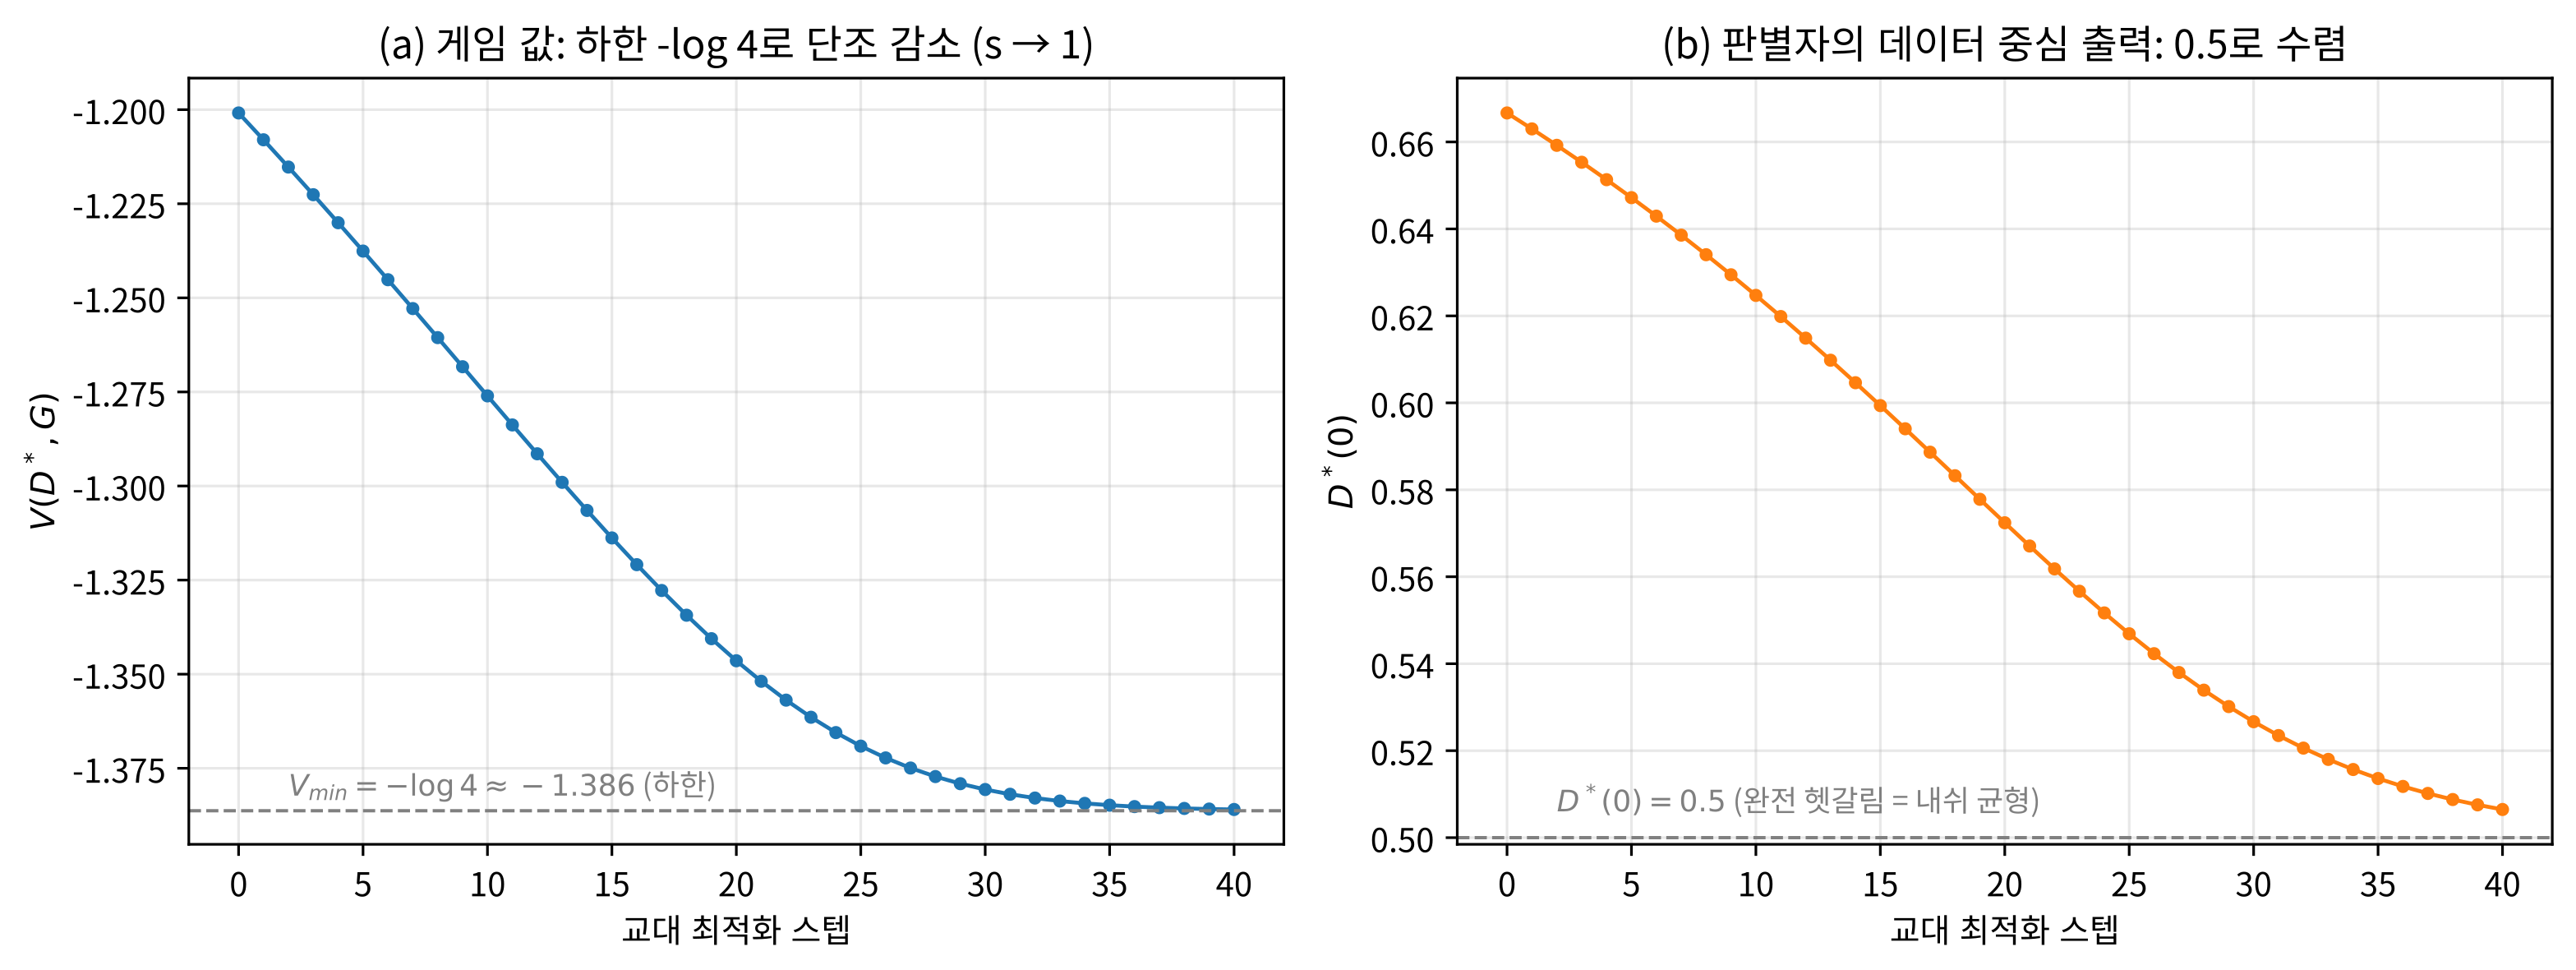
\includegraphics[width=\linewidth]{ch15_3_gan_dynamics.png}
      \vskip0.3em
      {\footnotesize 왼쪽: $V(D^*,G)$ 궤적, 오른쪽: $D^*(0)$ 수렴}
    \end{column}
  \end{columns}
\end{frame}

\begin{frame}{장난감의 한계: 평균을 못 움직임}
  \begin{itemize}
    \item 이 장난감의 생성자는 \textbf{평균을 못 움직임} → ``데이터의
      질량이 어디에 놓이는지''를 \textbf{선택할 자유가 없음} —
      너비만 맞출 뿐
    \item 일반적인 GAN의 생성자는 \textbf{이 자유까지} 갖고 있음
    \item \kq{모드 붕괴는 정확히 이 자유를 남용하는 실패 모드}
      (다음 섹션)
  \end{itemize}
\end{frame}

\begin{frame}{실전 학습: 교대 최적화의 함정}
  실제 GAN 학습 루프는 장난감과 같은 교대 구조 — 다만 닫힌 형태가
  없어서 ``최적 판별자로 점프'' 대신 \textbf{그라디언트 스텝}을 걸음.
  \begin{itemize}
    \item (1) 판별자 갱신: $G$ 고정, $D$만 한 스텝
    \item (2) 생성자 갱신: $D$ 고정, $G$만 한 스텝 — $G$\_loss의
      그래디언트가 $D$를 ``지나'' $G$의 파라미터로 흐름
    \item (두 번째 $fake$를 다시 계산하는 이유: 미분 그래프가
      \texttt{D.step()} 이후 \textbf{갱신된 $D$를 거쳐야} 생성자
      파라미터까지 흐름 — Ch.\,9 ``연산 그래프를 따라 거슬러 올라가는
      것'')
  \end{itemize}
  \vskip0.6em
  \begin{block}{EM과의 차이 (다시)}
    EM: E-step이 \textbf{정확한} 사후확률을 채워넣음 → ``우도가
    단조증가''가 \textbf{증명 가능}. GAN: (1)이 $D$를 완전 최적화하지도,
    (2)가 $G$를 완전 최적화하지도 못하는 \textbf{근사적} 게임 최적화
    → 학습 곡선이 ``꾸준히 하강하는 우도''처럼 보이지 않고, 오히려
    \textbf{등락을 거듭}.
  \end{block}
\end{frame}

\begin{frame}{불안정성의 세 가지 양상}
  \begin{itemize}
    \item \kb{$D$가 너무 강해지면 $G$의 그래디언트가 무용화} —
      $D$가 모든 가짜를 $D \approx 0$으로 확신하면, $\log(1 - D(G(z)))
      \approx 0$과 $\log D(G(z)) \to -\infty$ 사이에서 $G$가 받는
      신호는 ``네가 만든 건 전부 가짜''라는 \textbf{방향 없는 신호}
      → Ch.\,9 ``\textbf{그라디언트 소실}''과 정확히 같은 구조
    \item \kb{$D$가 너무 약하면 $G$는 ``약한 판별자만'' 속이는 법을
      배움} — $D$의 빈틈을 파고드는 가짜가 손실을 최소화하지만,
      데이터 분포 자체를 잘 본 것은 아님. $D$가 다음에 더 강해지면
      다시 무너짐.
    \item \kb{두 네트워크의 ``학습 속도 밸런스''가 중요} — 한쪽이
      너무 빨리 수렴하면 다른 쪽의 학습 신호가 사라짐. 실전 대응:
      $D$에 \textbf{배터치 정규화}(Ch.\,9)를 쓰거나, $G$에 학습률을
      작게 맞추거나, 그래디언트 페널티(WGAN-GP)를 붙이는 등
  \end{itemize}
\end{frame}

\begin{frame}{실수 1: D 정확도 50\%를 ``실패''로 읽기}
  \begin{block}{거꾸다}
    이 게임에서 $D$의 정확도 50\%는 \textbf{가장 이상적인 운영점}
    (내쉬 균형).
  \end{block}
  \vskip0.6em
  \begin{itemize}
    \item 학습 중 $D$의 정확도가 \textbf{50\% 부근}에서 머물면
      ``양쪽이 서로를 잘 따라가고 있다''는 \textbf{신호}
    \item 반대로 $D$의 정확도가 \textbf{90\%+}로 치솟으면
      \kq{$G$가 이미 학습에서 이탈한 전형적 실패 신호} — ``$D$가
      잘 learned하고 있다''가 아니라 \textbf{``$G$가 $D$를 못
      따라가고 있다''}는 뜻
  \end{itemize}
\end{frame}

\begin{frame}{모드 붕괴: ``성공''이 ``실패''가 되는 지점}
  \begin{itemize}
    \item 실전 GAN 학습이 자주 불안정 — 생성자가 판별자를 속이는
      \textbf{몇 가지 패턴에만 몰려} 다양성을 잃는 현상 =
      \kb{모드 붕괴(mode collapse)}
    \item VAE: 이론적으로 \textbf{안정적}이지만 생성 품질이 다소
      \textbf{흐릿}(blurry) 경향
    \item GAN: \textbf{선명한} 결과이지만 \textbf{학습이 까다로움}
  \end{itemize}
  \vskip0.6em
  \begin{block}{1차원 장난감이 이미 메커니즘을 보여줌}
    기본 GAN 목적함수에는 \textbf{``다양성을 유지하라는 항''이
    없음}. 생성자 손실 $-\log D(G(z))$는 오직 ``이 가짜가 $D$를
    얼마나 속였는가''에 의존. 데이터 분포가 세 개의 모드(예: 세
    종류의 동물)를 갖고 있어도, \textbf{하나의} 모드만 집중적으로
    만들어도 $D$를 잘 속일 수 있다면 — 고차원 공간에서 $D$가 ``세
    모드 모두를 동시에 감시''할 수 없는 한 — 그 하나에 집중하는 것이
    손실을 줄이는 \textbf{가장 확실한} 전략.
  \end{block}
\end{frame}

\begin{frame}{VAE에는 이 항이 있다: 핵심 구조적 차이}
  \begin{columns}[T]
    \begin{column}{0.5\textwidth}
      \kb{VAE (15.1절)}
      \begin{itemize}
        \item KL 항 $D_{KL}(q_\phi(z|x) \| p(z))$이 ``인코더 출력
          분포가 표준정규분포에 가깝게 유지''를 \textbf{목적함수 안에
          명시적으로} 요구
        \item 잠재 공간 \textbf{전체}가 쓰이는 구조적 압력
        \item ``잠재 공간의 일부만 쓰는'' 퇴화 = \textbf{ELBO를
          직접적으로 낮추는 행위}
      \end{itemize}
    \end{column}
    \begin{column}{0.5\textwidth}
      \kb{GAN}
      \begin{itemize}
        \item 내쉬 균형 $p_G = p_{\text{data}}$ (모든 모드를 덮는
          분포)가 ``완전한 균형''
        \item 실제 학습이 풀고 있는 \textbf{근사적} 게임에서는
          ``일부 모드를 덮고 $D$를 속이는'' 분포도 \textbf{국소적으로
          균형처럼} 작용
        \item 이 대응 \textbf{항이 없음}
      \end{itemize}
    \end{column}
  \end{columns}
  \vskip0.8em
  \kq{이것이 VAE/GAN 비교에서 반복되는 \textbf{핵심 구조적 차이}.}
\end{frame}

\begin{frame}{2014년 이후 GAN 계열: ``안정화''가 3년의 주제}
  기본 GAN의 불안정성을 고치려는 시도가 GAN 연구의 줄기를 이룸
  (각 방법의 정확한 수학은 넘기고, ``무엇을 고치려 했는지''만):
  \begin{itemize}
    \item \kb{WGAN / WGAN-GP (2017, Arjovsky et al.\ / Gulrajani et
      al.)} — ``$D$가 $G$를 완전히 이기면 $G$의 그래디언트가
      사라진다''는 문제를 정조준. 게임의 값을 두 분포의
      \textbf{워터스톤 거리}(Wasserstein-1, 두 분포를 ``이동시켜
      일치시키는 최소 비용'' — 어스무버 거리)로 바꾼 뒤, $D$를
      \textbf{1-Lipschitz}로 제한(처음엔 가중치 클리핑, WGAN-GP는
      \textbf{그래디언트 페널티}) → 게임 값이 두 분포의 실제 거리와
      일치해 $G$가 \textbf{분포가 어디로 옮겨가야 하는지 방향
      신호}를 계속 수신. 그래디언트가 ``0''으로 안 죽음 → 학습이
      훨씬 안정적, 모드 붕괴도 감소.
    \item \kb{pix2pix (2016), CycleGAN (2017)} — ``이미지 $\to$
      이미지'' 변환으로 확장. CycleGAN은 \textbf{레이블된} 데이터
      없이도 (말 사진만, 기린 사진만) 두 분포 사이의 대응을 학습해
      ``말 $\to$ 기린'' 같은 스타일 변환 — GAN이 ``비슷한 이미지
      생성''을 넘어 \textbf{구조를 보존하며 변환}하는 도구로 확장.
    \item \kb{StyleGAN (2018--2019)} — 초고해상도 합성 인간 얼굴.
      잠재 벡터를 ``스타일 수준별로'' 나눠 조작 → ``얼굴 표정만
      바꾸고 얼굴 형태는 그대로'' 같은 \textbf{제어된} 생성
      (16장 팀 프로젝트에서 다시 만남).
    \item \kb{BigGAN (2019)} — ImageNet 전체에 걸친 대규모
      \textbf{조건부} 생성 — ``이 클래스의 이미지를 만들어라''를
      1024$\times$1024 해상도로.
  \end{itemize}
  \vskip0.4em
  {\footnotesize 2016년 튜링상 연설에서 굿펠로우는 GAN을 ``딥러닝에서
  최근 몇 년간 가장 멋진 아이디어''라 말함 — 그 원본이 바로
  ``평균적 품질''이라 거절당한 그 논문.}
\end{frame}

\begin{frame}{Diffusion: 정방향/역방향 과정}
  \begin{block}{정방향 과정 (forward process)}
    진짜 이미지 $x_0$에 \textbf{아주 작은 노이즈를 $T$번 반복}해서
    추가해, 결국 $x_T$가 \textbf{순수한 무작위 노이즈}가 됨.
    \; 이 과정은 \textbf{고정된 절차이지 학습 대상이 아님}.
  \end{block}
  \vskip0.4em
  \begin{block}{역방향 과정 (reverse process)}
    신경망이 \textbf{``한 단계 전 노이즈가 어땠는지''}를 예측하도록
    학습. \; 학습 후, 순수 노이즈 $x_T$에서 시작해 이 역방향 단계를
    $T$번 반복 → \textbf{새로운 이미지}.
  \end{block}
  \vskip0.6em
  \begin{itemize}
    \item GAN이 ``\textbf{한 번에}'' 노이즈를 이미지로 바꾸려 하는
      것과 달리, Diffusion은 그 어려운 문제를 \textbf{아주 작은
      단계 $T$개로 잘게 쪼갬} — 각 단계는 ``노이즈를 아주 조금만
      제거''하는 훨씬 쉬운 문제 → \textbf{전체적으로 훨씬 안정적}
    \item \textbf{대가}: 이미지 하나 생성에 $T$번 반복 필요 → GAN보다
      \textbf{생성 속도 느림}
    \item 지금 가장 널리 쓰이는 이미지 생성 모델(Stable Diffusion
      등)이 이 원리 사용
  \end{itemize}
\end{frame}

\begin{frame}{정방향은 왜 ``학습 대상''이 아닌가}
  \begin{itemize}
    \item 정방향 과정은 \textbf{고정된, 알려진} 절차:
    \[x_t = \sqrt{1-\beta_t}\,x_{t-1} + \sqrt{\beta_t}\,\epsilon_t,
      \qquad \epsilon_t \sim \mathcal{N}(0, I)\]
    \item 각 단계에 ``얼마나 큰 노이즈를 추가하는지''가 미리 정해진
      \textbf{$\beta_t$ 스케줄}에 따라 기계적 진행
    \item 노이즈를 \textbf{추가하는} 것은 역산이 됨 — 정확한 노이즈
      값을 알면 $x_{t-1}$을 바로 구함
    \item ``어려운'' 부분은 \textbf{노이즈 값을 관측하지 못한} 상태에서
      ``이 상태 $x_t$에서 한 단계 전은 어땠을까''를 추측하는
      \textbf{역방향} 쪽
  \end{itemize}
  \vskip0.6em
  \begin{block}{학습 대상은 하나뿐}
    역방향 모델 $p_\theta(x_{t-1} \mid x_t)$.
  \end{block}
\end{frame}

\begin{frame}{``노이즈 예측'' 회귀 문제 (DDPM)}
  실전(DDPM)에서는 역방향 분포를 직접 매개변수화하지 않고, 대신
  신경망 $\epsilon_\theta(x_t, t)$가 \textbf{$x_t$에 추가된 노이즈
  $\epsilon_t$를 예측}하도록 학습:
  \[
  \mathcal{L}(\theta) =
  \mathbb{E}_{t, x_0, \epsilon}\left[
    \lVert \epsilon - \epsilon_\theta(x_t, t) \rVert^2
  \right]
  \]
  \vskip0.6em
  \begin{block}{이 식이 \textbf{MSE 회귀 손실}이라는 점에 주목}
    이 장에서 본 모든 방식(EM의 M-step, VAE의 ELBO 역전파)과 달리,
    GAN의 min-max 게임도 아니고, 우도의 적분 근사도 아닌,
    \textbf{가장 보통의 단일 회귀 최적화}.
    \; ``안정적으로 학습된다''의 \textbf{정체}가 바로 이것.
  \end{block}
  \vskip0.4em
  {\footnotesize 수학적으로 이 $\epsilon$ 예측은 $\nabla_x \log p_t(x)$,
  즉 데이터 분포의 \textbf{스코어 함수}를 추정하는 것과 동치
  (Song \& Ermon, 2019) — ``노이즈를 잘 예측'' = ``데이터가 어디에
  빽빽한지 그 기울기를 안다''.}
\end{frame}

\begin{frame}{역방향 단계(DDPM)와 ``다시 노이즈 추가''}
  역방향 단계는 한 줄:
  \[
  x_{t-1} = \frac{1}{\sqrt{\alpha_t}}\Big( x_t -
  \frac{1-\alpha_t}{\sqrt{1-\bar\alpha_t}}\,
  \epsilon_\theta(x_t,t) \Big) + \sigma_t\, z, \quad
  z \sim \mathcal{N}(0, I)
  \]
  \vskip0.6em
  \begin{itemize}
    \item ``$\epsilon_\theta$만큼 \textbf{빼고}(조금 깨끗해지고),
      $\sigma_t z$만큼 \textbf{다시 더한다}(다시 노이즈를 조금)''
    \item \textbf{역방향에도 노이즈를 다시 추가}하는 이 마지막 항이
      처음엔 의외로 보일 수 있음
    \item 이유: $x_{t-1} \mid x_t$가 ``\textbf{하나의 점}''이 아니라
      \textbf{가우시안 분포}(불확실성이 있는)이기 때문
    \item ``한 단계 전''도 \textbf{관측되지 않았으므로}, 그 분포에서
      샘플링하는 것이 \textbf{절차의 일부}
  \end{itemize}
  \vskip0.6em
  \begin{block}{자주 하는 실수 3}
    ``denoise = 계속 깨끗해지는 과정''이라는 직관과 달리, DDPM의
    역방향 단계에는 $+\sigma_t z$(\textbf{다시 노이즈 추가})가
    있음. 이 항을 빼면 역방향 과정이 더 이상 $p(x_{t-1}\mid x_t)$
    가 아니라 \textbf{``점 추정''}으로 바뀌고, 생성 품질이 크게
    떨어짐. $x_{t-1} \mid x_t$가 \textbf{분포}라는 점을 잊지 말 것.
  \end{block}
\end{frame}

\begin{frame}{역사: Sohl-Dickstein 2015 $\to$ DDPM 2020}
  \begin{itemize}
    \item 2015년 \kb{Sohl-Dickstein} 외 ``Deep Unsupervised Learning
      using Nonequilibrium Thermodynamics'' — 정방향/역방향 아이디어
      \textbf{처음 딥러닝에 제안}. 하지만 \textbf{학습이 너무 느려}
      실용화 못 함
    \item 2020년 \kb{DDPM} (Ho, Jain \& Abbeel, ``Denoising
      Diffusion Probabilistic Models''):
      (i) 노이즈 예측 매개변수화 $\epsilon_\theta$,
      (ii) 단순한 MSE 손실,
      (iii) 실용적 스케줄
      → \textbf{실제로 쓸 만한} 알고리즘으로 만듦
    \item 같은 해 \kb{DDIM} (Song et al.): 역방향 과정을
      \textbf{거의 결정적으로} 만들어 $T$를 \textbf{1000에서 약 50}
      단계로 줄임
    \item 2022년 \kb{Stable Diffusion} (Stability AI): 여기에 15.1절의
      \textbf{VAE}를 조합 — 이미지를 VAE 인코더로 \textbf{8$\times$
      압축한 잠재 공간}에서 Diffusion을 돌림, 계산량 $1/8^2$로
      감소
    \item 15.1에서 ``VAE의 매끄러운 잠재 공간''이 왜 중요한지 —
      그것이 곧 Diffusion을 \textbf{안정 있게} 학습·추론할 수 있게
      하는 \textbf{전제 조건}
    \item 같은 해 DALL$\cdot$E 2, Midjourney, 2024년 Sora(영상)까지
      — 이미지 생성의 \textbf{주류가 Diffusion으로 이동}
  \end{itemize}
  \vskip0.5em
  \kq{세 원리가 각자 독립적으로 끝나는 것이 아니라 \textbf{서로
  연결}되어 실전 시스템으로 합쳐진다는 점 — 이번 장을 ``세 개를
  나란히'' 보는 이유.}
\end{frame}

\begin{frame}{GAN vs Diffusion: ``학습할 것'' 한 줄}
  \small
  \begin{tabular}{@{}p{0.28\textwidth}p{0.32\textwidth}p{0.32\textwidth}@{}}
    \toprule
     & GAN & Diffusion \\
    \midrule
    학습할 네트워크 & 2개 ($G, D$) & 1개 ($\epsilon_\theta$) \\
    학습 목표 & 게임의 \textbf{균형}(닫힌 형태 없음) &
      $\lVert\epsilon - \epsilon_\theta\rVert^2$ (\textbf{MSE}) \\
    샘플링 시 순전파 & \textbf{1회} & $T$회 (DDIM으로 $\sim$50회) \\
    \bottomrule
  \end{tabular}
\end{frame}

\begin{frame}{이미지 밖으로: Waymo SceneDiffuser}
  Diffusion의 ``노이즈를 점진적으로 되돌린다''는 원리는 픽셀 공간에
  머물지 않음.
  \begin{itemize}
    \item 2024년 \kb{Waymo} 자율주행 개발 시뮬레이션 도구
      \kb{SceneDiffuser}:
      \textbf{자연어 지시}(``자신의 차가 저속 차량을 따라가는
      장면'' 같은)로부터 \textbf{3차원 교통 장면의 초기 배치}(차량·
      보행객의 위치, 진행 방향, 크기)를 생성 + 그 장면을
      \textbf{앞으로 전개될 미래(롤아웃)}까지 시뮬레이션
    \item 핵심: ``\textbf{장면 수준(scene-level)의 Diffusion
      사전분포}'' — 장면 전체 상태가 시간에 따라 어떻게 흘러갈지를
      하나의 \textbf{스페이오-템포럴(spatio-temporal, 공간-시간)}
      Diffusion 모델로 예측
    \item roadgraph·교통 신호 같은 제약 조건으로 노이즈 제거를 유도하는
      \textbf{조건부 생성} — Stable Diffusion의 ``텍스트 $\to$
      이미지''와 \textbf{정확히 같은 패턴}
    \item Stable Diffusion이 \textbf{이미지 하나}의 잠재 공간에서
      노이즈를 되돌렸다면, SceneDiffuser는 \textbf{시간을 축으로 한
      장면 전체}에서 되돌림
    \item $\Rightarrow$ 자율주행 시스템을 테스트할 \textbf{상상 속
      시나리오}를 대량으로 생성 — ``\textbf{생성 모델이 안전 검증
      도구로 쓰인다}''는 점을 보여주는 대표 사례.
      추론에 필요한 모델 호출 횟수도 \textbf{16배} 감소
  \end{itemize}
\end{frame}

\begin{frame}{세 원리 비교}
  \small
  \begin{tabular}{@{}p{0.22\textwidth}p{0.26\textwidth}p{0.26\textwidth}p{0.26\textwidth}@{}}
    \toprule
     & VAE (우도 기반) & GAN (적대적) & Diffusion (스코어 기반) \\
    \midrule
    잠재변수 & 연속 \textbf{벡터} & \textbf{없음}(노이즈를 직접 변환)
      & 연속(노이즈 \textbf{단계}) \\
    학습 방법 & ELBO \textbf{최대화}(역전파) & \textbf{min-max 게임}의
      균형 & 각 단계 \textbf{노이즈 예측} 오차 최소화 \\
    학습 안정성 & \textbf{비교적 안정적} & \textbf{불안정하기 쉬움}
      & \textbf{안정적} \\
    생성 속도 & \textbf{빠름}(한 번에) & \textbf{빠름}(한 번에)
      & \textbf{느림}(반복 필요) \\
    \bottomrule
  \end{tabular}
  \vskip0.8em
  {\footnotesize 참고: 4.4절 GMM도 같은 질문의 \textbf{이산 잠재변수}
  버전 — $z$가 클러스터 번호라 E-step이 닫힌 형태로 \textbf{정확히}
  계산되므로, ``정밀하지만 이산''으로 여기 추가하지 않음.}
\end{frame}

\begin{frame}{잠재변수 행 다시 읽기}
  ``관측 안 된 구조''가 세 방식에서 각각 무엇이었는지:
  \begin{itemize}
    \item \kb{VAE}의 $z$ = \textbf{연속 벡터} — 가능치가 무한해서
      E-step을 신경망으로 \textbf{근사}해야 함 (15.1절)
    \item \kb{GAN}의 $z$ = \textbf{분포가 아니라 그냥 랜덤 입력} —
      ``데이터를 설명하는 잠재변수''의 역할을 \textbf{하지 않고},
      생성자가 입력으로 받는 \textbf{다양성의 원천}일 뿐
      ($z$의 분포를 학습하지도, $z \mid x$를 추론하지도 않음)
    \item \kb{Diffusion}의 ``잠재변수'' = \textbf{중간 상태 $x_t$}
      — 연속적이지만 \textbf{단계 $t$가 이산적으로 $T$개인},
      ``점진적으로 오염된 데이터'' 그 자체
  \end{itemize}
\end{frame}

\begin{frame}{학습 방법 행 다시 읽기: 안정성의 원인}
  \begin{itemize}
    \item \kb{VAE}: ELBO(단일 목적함수)를 역전파로 최대화하는
      \textbf{보통의} 최적화 → \textbf{안정}
    \item \kb{Diffusion}: MSE 회귀라 \textbf{가장 보통의} 최적화 →
      \textbf{안정}
    \item (대조: 4.4절 EM은 \textbf{닫힌 형태}의 좌표별 최적화라
      \textbf{증명 가능하게} 안정)
    \item \kb{GAN}: \textbf{두 개의 최적화 알고리즘이 서로의
      목표함수를 바꾸어놓는} 게임 — \textbf{단조증가도, 볼록성도,
      ``수렴했다는 것'' 자체의 정의}도 — 안정성의 \textbf{근거가
      없음}
  \end{itemize}
\end{frame}

\begin{frame}{생성 속도 행: ``안정성의 대가''}
  \begin{itemize}
    \item 가장 \textbf{안정한} Diffusion은 생성에 \textbf{$T$회
      반복} 필요 (DDIM으로 줄여도 수십 회)
    \item 가장 \textbf{빠른} GAN/VAE는 \textbf{한 번의} 순전파로 생성
  \end{itemize}
  \vskip0.8em
  \begin{block}{장 전체를 관통하는 트레이드오프}
    ``\textbf{데이터를 설명할 수 있다}(안정성, 평가 가능)'' vs
    ``\textbf{빨리 만들 수 있다}(속도)''
  \end{block}
  \vskip0.6em
  \begin{block}{실전 시스템은 ``하나씩 고르는 것''이 아니라 \textbf{조합}}
    Stable Diffusion = \kb{VAE}(잠재 공간) $\times$
    \kb{Diffusion}(노이즈 제거). \;
    SceneDiffuser = \kb{Diffusion} 원리를 \textbf{시간 축의 장면}으로
    확장. \; $\Rightarrow$ ``세 원리를 나란히 보고 나서야,
    ``관측되지 않은 구조가 데이터를 만들어낸다''는 하나의 질문이
    얼마나 다양한 방식으로 풀릴 수 있는지''가 보임.
  \end{block}
\end{frame}

\begin{frame}{자주 하는 실수 2·4: GAN/Diffusion 판독}
  \begin{block}{실수 2 — ``생성자의 loss가 계속 줄어야 정상''이라고
  기대}
    GAN의 loss 곡선은 \textbf{등락} — $D$가 갱신될 때마다 $G$의
    손실 함수 \textbf{자체}가 바뀌므로, ``loss가 튀었다''가 반드시
    실패를 뜻하지 않음. (반대로 EM의 우도처럼 \textbf{단조증가}하는
    곡선을 기대하면 GAN의 ``정상''을 ``이상''으로 오독.)
    \; 실전에서는 \textbf{샘플 품질}을 직접 보고, $D$의 정확도가
    50\% 부근에서 \textbf{균형}을 유지하는지를 대시보드로.
  \end{block}
  \vskip0.4em
  \begin{block}{실수 4 — ``$D$의 정확도 50\%''를 ``잘 안 하고
  있다''로 읽기}
    \textbf{반대}다 — 50\%는 이 게임의 \textbf{목표} operating
    point(내쉬 균형). \textbf{정확도가 90\%+로 치솟는 쪽}이 진짜
    문제 신호 (위 ``실전 학습''의 실수 1 참고).
  \end{block}
\end{frame}

\begin{frame}{확인 문제 (15.2)}
  \begin{enumerate}
    \item \textbf{(손계산, Tier A)} 1차원 장난감 GAN에서 $\mu = 0.5$
      일 때 게임의 값 $V(D^*, G) = \log(1 + 1/\phi(0.5))$를 계산
      ($\phi(0.5) = 0.3521$). 균형점 $\mu = 0$에서의 값
      $V(D^*, G) = \log(1 + 1/\phi(0)) = \log(1 + 1/0.3989)$와
      비교 — ``$\mu = 0.5$에서는 아직 균형이 아니며, 생성자는
      $\mu$를 어떤 방향으로 움직일 유인이 있는가''를 한 문장으로
      (힌트: $\mu = 0$에서의 값이 \textbf{더 작아야} $\mu = 0$이
      $G$의 최소 — 즉 $G$의 관점의 내쉬 균형).
    \item \textbf{(개념 서술)} 1차원 장난감에서 생성자는 결국
      $\mu = 0$ \textbf{하나의 점}을 만듦 — 게임 관점에서는
      ``판별자를 완전히 속였다''의 \textbf{성공}이지만, 생성
      품질 관점에서는 ``다양성 0''의 \textbf{실패}. VAE의 ELBO에는
      이 문제를 막는 \textbf{명시적인 항}이 있는데, 그 항이 무엇이며
      GAN의 목적함수에는 왜 대응하는 항이 없는지를 두세 문장.
  \end{enumerate}
\end{frame}

\begin{frame}{자주 묻는 질문: 모드 붕괴 · VAE/GAN/Diffusion}
  \begin{block}{모드 붕괴는 왜 생기나요?}
    생성자는 판별자를 속이기만 하면 손실이 줄어듦 — 어떤 \textbf{한
    종류}의 가짜가 판별자를 아주 잘 속인다는 것을 발견하면, 굳이
    다른 다양한 가짜를 만들 이유가 없음. 판별자가 그 ``치팅''을
    알아채고 대응하기 전까지, 생성자는 그 \textbf{좁은 영역에만
    몰릴} 유인. \; 근본 원인: VAE의 ELBO처럼 ``\textbf{다양성을
    명시적으로 요구하는 항}''이 GAN 기본 목적함수에는 \textbf{없음}.
  \end{block}
  \vskip0.4em
  \begin{block}{Diffusion이 주류인데 VAE·GAN은 이제 안 쓰나요?}
    이미지 생성 분야에서는 Diffusion이 최근 주류가 됐지만,
    \textbf{VAE의 핵심 아이디어}(잠재 공간을 매끄럽게 만든다)는
    여러 최신 시스템에서 Diffusion과 \textbf{결합}되어 사용
    (예: 픽셀 공간이 아니라 \textbf{VAE로 압축한 잠재 공간}에서
    Diffusion을 돌리는 구조 — Stable Diffusion이 정확히 이 방식).
    \; GAN도 \textbf{실시간성}이 중요한(반복 없이 한 번에 생성해야
    하는) 응용에서는 여전히 사용 — ``하나가 다른 셋을 완전히
    대체했다''기보다, \textbf{각자 강점이 있는 도구로 함께}.
  \end{block}
\end{frame}

\begin{frame}{자주 묻는 질문: Diffusion 단계 수 · GAN 평가}
  \begin{block}{Diffusion은 정말 $T$번의 단계를 다 돌리나요?}
    원래 DDPM은 $T = 1000$인데, \kb{DDIM}(2020)이 역방향 과정을
    거의 \textbf{결정적}으로 만들어 \textbf{약 50단계}로 줄이고,
    이후 \textbf{증류}(distillation) 계열 기법(\kb{LCM},
    \kb{progressive distillation} 등)으로 \textbf{10단계 이하}
    가능. \; 대가 = ``완전한 DDPM에 비하면 품질이 조금
    떨어짐''. \; ``GAN보다 느리다''는 GAN 기준에서 \textbf{상대적} —
    50단계 $\times$ 0.1초 $\approx$ 5초의 이미지 생성은 실제 응용에
    \textbf{충분히 빠름}. (영상 생성처럼 샘플 수백 장을 만들어야
    하는 분야에서는 이 차이가 더 중요.)
  \end{block}
  \vskip0.4em
  \begin{block}{GAN은 ELBO 같은 ``높을수록 좋은 단일 숫자''가 없는데,
  학습 품질을 어떻게 평가?}
    GAN 계열은 단일 ``우도'' 숫자가 없어서 \textbf{샘플 기반} 지표가
    따로 발전 — 대표적으로 \kb{FID}(Fréchet Inception Distance):
    실제 이미지와 생성 이미지를 InceptionNet 같은 \textbf{특징
    추출기}로 변환한 뒤, 두 특징 분포의 \textbf{평균·공분산}(가우시안
    근사) 사이의 \textbf{거리}. \; FID가 \textbf{작을수록} 생성
    분포가 실제 분포에 \textbf{가깝}. \; VAE/GMM 계열은 ``ELBO를
    높인다''는 단일 숫자가 있어 비교가 쉬웠는데, GAN은 FID처럼
    \textbf{외부 지표}가 필요 — 이(하나의 요인)가 이후 연구가
    ``\textbf{평가 가능한}'' Diffusion 쪽으로 이동하는 데 일조.
  \end{block}
\end{frame}

\begin{frame}{연습문제 (코딩)}
  \begin{itemize}
    \item \textbf{1.} \texttt{em\_step}과
      \texttt{kl\_divergence\_gaussian}(정규분포
      $\mathcal{N}(\mu, \sigma^2)$와 표준정규분포 사이의 KL
      divergence) 완성. \; 핵심 줄:
      $D_{KL} = -0.5 \cdot (1 + \texttt{log\_var} - \mu^2
      - \exp(\texttt{log\_var}))$.
    \item \textbf{2.} \texttt{discriminator\_loss}와
      \texttt{generator\_loss} 완성 (위 15.2 절의 코드를 참고).
    \item \textbf{3.} (개념) GMM에서 각 클러스터의 분산을 아주
      작은 값으로 \textbf{고정}하고 학습하지 않으면 왜
      \textbf{k-means와 같아지는지} 설명하고, VAE(우도 기반)와
      GAN(적대적)의 \textbf{생성 품질·학습 안정성 트레이드오프}를
      두세 문장으로 비교.
    \item \textbf{4.} (손유도, Tier B) 데이터 3개
      $x_1 = 1, x_2 = 9, x_3 = 10$, 2개 클러스터, 현재 파라미터
      $\mu_1 = 0, \sigma_1 = 1, \mu_2 = 9, \sigma_2 = 1,
      \pi_1 = \pi_2 = 0.5$. $x_1$에 대한 \textbf{책임값}
      $\gamma_{1,1}$과 $\gamma_{1,2}$를 손으로 계산 (힌트: 정규
      밀도를 $x_1 = 1$에 대해 두 클러스터 각각 계산 후 대입.
      $\pi_1 = \pi_2$이므로 실제로는 $\pi$가 \textbf{약분}되어
      사라짐).
    \item \textbf{5.} (손유도, Tier C — 폴백 준비 대상)
      $\log p_\theta(x) = \log \int p_\theta(x,z)\,dz$에서 시작해
      옌센 부등식($\log \mathbb{E}[X] \ge \mathbb{E}[\log X]$)을
      이용해 15.1절의 ELBO 부등식을 유도.
  \end{itemize}
\end{frame}

\begin{frame}[fragile]{연습문제 5: ELBO 유도 빈칸 폴백}
  \textbf{자유 유도가 어려운 경우} — 빈칸을 채워라:
\begin{lstlisting}
Step 1: log p(x) = log integral[ q(z|x) * (p(x,z) / q(z|x)) dz ]
                  = log E_q[ ______________ ]

Step 2: 옌센 부등식(log가 오목함수) 적용:
  log E_q[ p(x,z)/q(z|x) ] >= E_q[ log(______________) ]

Step 3: p(x,z) = p(x|z) * p(z)로 분해하면:
  = E_q[ log p(x|z) ] + E_q[ ______________ ]

Step 4: E_q[ log p(z) - log q(z|x) ] = -D_KL(q(z|x) || p(z))

결론: log p(x) >= E_q[log p(x|z)] - D_KL(q(z|x) || p(z))   [ELBO]
\end{lstlisting}
  \vskip0.4em
  \begin{block}{정확성 확인}
    Step 2에서 \textbf{부등호가 등호가 아니라 부등식}인 이유를 한
    문장으로 — (옌센 부등식이 \textbf{언제 등식}이 되는지:
    $X$가 \textbf{상수}일 때).
  \end{block}
\end{frame}

\begin{frame}{이번 주차 정리}
  \begin{enumerate}
    \item \kb{15.1 VAE} — \textbf{``EM의 E-step을 신경망이 맡는다''}.
      ELBO = \textbf{복원 항} $-$ \textbf{KL 정규화 항} (옌센 부등식
      한 번으로 유도). \; 갭 $= D_{KL}(q \| p(z|x))$ — ELBO
      최대화 $=$ 변분 베이즈. \; \textbf{$\mu^2$ 항}이 인코더 위치를
      원점 쪽으로, \textbf{$\sigma^2$ 항}이 너비를 제어. \;
      \textbf{생성 모드}는 인코더를 \textbf{버리고} 디코더만 통과.
      \; $\beta$-VAE가 ``복원 품질 vs 잠재 공간 매끄러움''을
      튜닝. \; ``흐릿함''의 원인 = \textbf{기대값 최적화}.
    \item \kb{15.2 GAN} — min-max 게임의 \textbf{내쉬 균형}
      ($D(x) = 0.5$, $p_G = p_{\text{data}}$). \; 1차원 장난감에서
      $V(D^*, G) = 2\,\mathrm{JSD} - \log 4$로 \textbf{닫힌
      형태}. \; 성공 신호 = $V$가 $-\log 4$ 근방에서 \textbf{안정},
      $D^*(0) \to 0.5$. \; \textbf{모드 붕괴}의 원인 = 목적함수에
      \textbf{다양성 항이 없음} (VAE에는 KL 항이 대응). \;
      WGAN/CycleGAN/StyleGAN/BigGAN = ``\textbf{안정화}''가 3년의
      주제.
    \item \kb{15.2 Diffusion + 비교} — 노이즈를 $T$단계로 \textbf{쪼갠
      MSE 회귀}(가장 보통의 최적화 → \textbf{안정}). \; 역방향에도
      $+\sigma_t z$(\textbf{다시 노이즈 추가})가 \textbf{필요}.
      \; Stable Diffusion = \textbf{VAE 잠재 공간} $\times$
      Diffusion. \; 세 원리: \textbf{잠재변수 · 학습 방법 · 안정성 ·
      생성 속도}로 비교 — 실전 시스템은 \textbf{조합}.
  \end{enumerate}
  \vskip0.6em
  \begin{block}{다음 주 — Chapter 16. Block B 캡스톤: 팀 프로젝트와
  ML1 총정리}
    이번 장에서 배운 \textbf{세 원리(VAE·GAN·Diffusion)}가 팀
    프로젝트의 \textbf{모델 선택} 도구 상자로 등장 —
    \textbf{안정성 · 생성 속도 · 품질}의 기준으로 선택하고
    \textbf{정당화}.
  \end{block}
\end{frame}

\end{document}
